\documentclass[12pt,fleqn,openany,oneside,showtrims]{memoir}

\usepackage{xr-hyper}
\usepackage[bookmarksopen,
            pagebackref=true,
            colorlinks,
            urlcolor=darkblue,
            linkcolor=darkblue,
            citecolor=darkblue,
            pdfauthor={Andrew W. Appel},
            pdftitle={Program Logics for Certified Compilers},
            pdfsubject={Computer Science},
            linktoc=all
            ]{hyperref}
\renewcommand{\chapterautorefname}{Chapter}

% Choose a font.  Bitstream Charter is readable in small formats / low res.
%\usepackage[bitstream-charter]{mathdesign}
% Other fonts I tried...
\usepackage{fouriernc}  % New Century Schoolbook is good too
\usepackage{amsfonts}  % New Century Schoolbook is good too
%\usepackage{lmodern}
%\usepackage{tgschola}
%\usepackage{fourier}
\usepackage[T1]{fontenc}

% The following stocksize and typeblock size has the following properties:
%  1. aspect ratio 165x133 works well on Kindle
%  2. trimmedsize does not matter for Kindle, but these tiny margins
%     will display well in Adobe Acrobat
%  Simple headers, no footers for good display on tablets and in Acrobat
\setstocksize{210mm}{153mm}
\settrimmedsize{\stockheight}{\stockwidth}{*}
\settypeblocksize{175mm}{133mm}{*}
\setlrmargins{*}{*}{1}
\setulmargins{*}{*}{1}
\setlength{\footskip}{0mm}
\setlength{\headsep}{5mm}
\setlength{\headheight}{7mm}
\checkandfixthelayout

% Adjust appearance of table of contents for compactness
\setlength{\cftpartnumwidth}{3em}
\setlength{\cftbeforepartskip}{2ex}
\setlength{\cftbeforechapterskip}{1pt}

% Very simple page headings, good on tablets/Kindle/Acrobat
\pagestyle{myheadings}
\makeoddhead{myheadings}{\textsc{\leftmark}}{}{\thepage}
\makeoddhead{plain}{}{}{\thepage}
\makeoddfoot{plain}{}{}{}

% Tone down the size of chapter titles and section headings
\renewcommand{\secheadstyle}{\large\itshape\bfseries}
\renewcommand{\chapnamefont}{\huge\itshape}
\renewcommand{\chaptitlefont}{\huge\itshape}
\renewcommand{\chapnumfont}{\huge\itshape}
\renewcommand{\partnamefont}{\huge\itshape\bfseries}
\renewcommand{\parttitlefont}{\huge\itshape\bfseries}
\renewcommand{\partnumfont}{\huge\itshape\bfseries}

% Adjust paragraph style
\raggedyright
\setlength{\ragrparindent}{2em}
\traditionalparskip
%\setlength{\parindent}{2em}

% I think this is supposed to make things more searchable in PDF files
\input glyphtounicode
\pdfgentounicode=1

% Set bounding box for good viewing on Kindle
\usepackage{color}
\definecolor{almostwhite}{gray}{0.98}
\renewcommand*{\trimmarkscolor}{\color{almostwhite}}
\renewcommand\tmarktl{}
\renewcommand\tmarktr{}
\renewcommand\tmarkbl{}
\renewcommand\tmarkbr{}
\renewcommand\tmarktm{
  \begin{picture}(0,0)
   \setlength{\unitlength}{1mm}\thicklines
    \put(0,-18){\line(10,0){10}}
  \end{picture}}
\renewcommand\tmarkbm{
  \begin{picture}(0,0)
   \setlength{\unitlength}{1mm}\thicklines
    \put(0,6){\line(10,0){10}}
  \end{picture}}
\renewcommand\tmarkmr{
  \begin{picture}(0,0)
   \setlength{\unitlength}{1mm}\thicklines
    \put(-10,0){\line(0,10){10}}
  \end{picture}}
\renewcommand\tmarkml{
  \begin{picture}(0,0)
   \setlength{\unitlength}{1mm}\thicklines
    \put(9,0){\line(0,10){10}}
  \end{picture}}
%\showtrimson  % Maybe this line is not necessary?

\bibliographystyle{plain}


\newcommand\newthought[1]{%
   \addvspace{0\baselineskip plus 0.5ex minus 0.2ex}%
   \noindent\textsc{#1}%
}

\usepackage[pdftex]{pict2e}
\usepackage[nocenter]{qtree}
\usepackage[fleqn]{amsmath}
%\usepackage{amssymb}  % DON'T NEED THIS WITH  \usepackage[...]{mathdesign}
\usepackage{mathpartir}
\usepackage{semantic}
\usepackage{stmaryrd}
\usepackage{bussproofs}
\usepackage{overlay}
\usepackage{caption}
\usepackage{stackrel}
\usepackage{mathtools}
%\usepackage{txfonts} % just for \boxdotright
\usepackage[normalem]{ulem}

\definecolor{darkblue}{rgb}{0,0.08,0.71}
\definecolor{darkred}{rgb}{0.5,0,0}


%\usepackage{microtype}

\usepackage{listings}
\usepackage{lstlangcoq}
\renewcommand{\lstlistingname}{Figure}
\lstset{language=Coq,basicstyle=\sffamily,mathescape=true,columns=fullflexible}

\usepackage{booktabs}  % For nicely typeset tabular material

\usepackage[pdftex]{graphicx}
\graphicspath{{graphics/}}
%%
% Prints a trailing space in a smart way.
\usepackage{xspace}

% Prints the month name (e.g., January) and the year (e.g., 2008)
\newcommand{\monthyear}{%
  \ifcase\month\or January\or February\or March\or April\or May\or June\or
  July\or August\or September\or October\or November\or
  December\fi\space\number\year
}


\usepackage{units}

% Typesets the font size, leading, and measure in the form of 10/12x26 pc.

\usepackage{makeidx}
\setsecnumdepth{chapter}
\setcounter{tocdepth}{0}



% Disclaimer for cover page (only for draft mode)

\newcommand\chapterfilemark{}
\newcommand\coverdisclaimer{}

\iffalse % cover page for prepublication draft
% latex-file-name marking at top right (only for draft mode)
\renewcommand{\chapterfilemark}{{\textcolor{red}\thefile}\hspace*{2em}}
\renewcommand\coverdisclaimer{
\parbox{2in}{\normalsize\textcolor{darkred}{
PREPUBLICATION DRAFT.\\
\today\\
DO NOT REDISTRIBUTE \\
without permission \\ from the author.}}}
\fi
\iffalse % cover page for sample chapter
\renewcommand{\chapterfilemark}{}
\renewcommand\coverdisclaimer{
\parbox{2in}{\normalsize\textcolor{darkred}{
TABLE OF CONTENTS \\
and SAMPLE CHAPTER\\
of prepublication \\
manuscript\\
\today \\
~\\}}}
\fi

% A few hacks for showing index entries in draft mode
%\setmarginnotes{20pt}{50pt}{10pt}
%\let\OldIndex\index
%\renewcommand{\index}[1]{{\textcolor{darkred}#1}\OldIndex{xx#1}}
% end of ``A few hacks''

\newcommand*{\xchapter}[1]{\refstepcounter{chapter}
  \ \newline
    {\rmfamily\itshape\Large\thechapter\hspace{1em} #1 }
  \newline
  \addcontentsline{toc}{chapter}{\protect\numberline{\thechapter}#1}}

\newcommand*{\xpart}[1]{\refstepcounter{part}
  \par\vspace*{20pt}
  \noindent
    {\rmfamily\itshape\huge PART~\thepart\hspace{1em} #1 }
  \newline
  \addcontentsline{toc}{part}{\protect\numberline{\thepart}#1}}

\newsavebox{\mybox}

\newcommand\thefile{}
\newcommand\includex[1]{\renewcommand\thefile{\small\textsf{#1}}\include{#1}}

\renewcommand{\_}{\texttt{\textunderscore}}

\newcommand{\measure}[3]{#1/#2$\times$\unit[#3]{pc}}

\newcommand{\hairsp}{\hspace{1pt}}% hair space
\newcommand{\ie}{\mbox{\textit{i.\hairsp{}e.}}\xspace}
\newcommand{\eg}{\mbox{\textit{e.\hairsp{}g.}}\xspace}
\newcommand{\opcit}{\emph{op. cit.}}

\newcommand{\emp}{\mathsf{emp}}
\newcommand{\subtype}{\hspace{1pt}\includegraphics[width=1em]{Tailrightarrow.pdf}\,}
\newcommand\rtarrow{\hspace{-.4ex}\rightarrow\hspace{-.5ex}}

\DeclareRobustCommand\longrightarrow
     {\relbar\mathrel{\mkern-4mu}\rightarrow}

\DeclareRobustCommand
  \longmapsto{\mapstochar\longrightarrow}


\renewcommand{\mapsto}{\,
\includegraphics[width=.9em, trim=0 0 0 3]{mapsto.pdf}\,}
\newcommand{\lbul}{
\includegraphics[width=.44em, trim=0 0 0 3]{lbul.pdf}\,}
\newcommand{\rbul}{
\includegraphics[width=.44em, trim=0 0 0 3]{rbul.pdf}\,}

\newcommand{\triple}[3]{\{#1\}\,#2\,\{#3\}}
\mathlig{|->}{\mapsto}
\newcommand{\later}{\triangleright}
%\newcommand{\wand}{\mathrel{\relbar\joinrel\!\!\relbar\!\!\!\ast\,}}
\newcommand{\wand}{\mathrel{-\hspace{-.7ex}*}}
\newcommand{\ewand}{\mathrel{-\hspace{-.42ex}\circ}}
%\newcommand{\ewand}{\multimap}
\newcommand{\TT}{\ensuremath{\mathsf{TT}}}
\newcommand{\FF}{\ensuremath{\mathsf{FF}}}
\newcommand{\EX}{\ensuremath{\mathsf{EX}\ }}
\renewcommand{\models}{\mathrel{|}\hspace{-.1ex}\joinrel\Relbar}
%\newcommand\guards{\raisebox{-.3ex}{\makebox[0pt][l]{$\sqcup$}}\raisebox{.2ex}{$\sqcap$}}
\newcommand\guards[2]{\{#1\}\hairsp #2}
\newcommand\semaxfunc[3]{#1\vdash_\mathrm{func} #2:#3}
\newcommand\pair[2]{\left<#1,#2\right>}
\newcommand{\boxdotright}{\!\mathrel\boxdot\joinrel\rightarrow\!}
\newcommand{\islock}{\boxdotright}
\newcommand{\islocksh}[1]{\stackrel{#1}\boxdotright}
\newcommand{\nxt}[2]{\mathsf{next}\,#1\,#2}
\newcommand{\lseg}[2]{#1\!\! \leadsto \!\!#2}
\newcommand\EVAL[2]{[\hspace{-.25em}[ #1 ]\hspace{-.25em}]_#2}
\newcommand{\listrep}[3]{#2 \stackrel{#1}{\leadsto} #3}
\newcommand{\listrepsh}[4]{#3 \stackrel{#2}{\leadsto}_{#1} #4}
\newcommand{\capar}[1]{~{\scriptsize #1:}}
\newcommand{\typecheck}[2]{#1 \vdash_\mathrm{type} #2}
\newcommand{\expcheck}[2]{#1 \vdash_\mathrm{exp} #2}

\newcommand{\andp}{\ensuremath{\,\mathsf{\&\hspace{-.2em}\&}\,}}
\newcommand{\orp}{\ensuremath{\,\|\,}}
\newcommand{\imp}{\ensuremath{\longrightarrow}}
\newcommand{\prop}{\ensuremath{!!}}
\newcommand\fash{\ensuremath{\#}}
\newcommand{\unfash}{!}

\newcommand{\PROP}{\mbox{\small PROP}}
\newcommand{\LOCAL}{\mbox{\small LOCAL}}
\newcommand{\PARAMS}{\mbox{\small PARAMS}}
\newcommand{\GLOBALS}{\mbox{\small GLOBALS}}
\newcommand{\SEP}{\mbox{\small SEP}}


\newcommand\oo{\circ}
\newcommand\Prop{\mathsf{Prop}}

\newcommand{\file}[1]{\mbox{\textsf{#1}}\index{#1@\textsf{#1}}}
\newcommand{\idef}[1]{\mbox{\textsf{#1}}\index{#1@\textsf{#1}}}
\newcommand{\iref}[1]{\mbox{\textsf{#1}}\index{#1@\textsf{#1}}}
\newcommand{\indexx}[1]{#1\index{#1}}
\newcommand{\indexy}[1]{\index{#1}}

\IfFileExists{redindex.tex}{\input{redindex.tex}}{}

\newcommand{\defeq}{~\mathsf{:=}~}
\renewenvironment{prooftree}%
{\par \vskip2ex plus.8ex minus.4ex}%
{\DisplayProof \par  \vskip2ex plus.8ex minus.4ex }

%% Set up the Qtree stuff
\renewcommand{\qtreepadding}{2pt}
\renewcommand{\qtreeunaryht}{0.5em}
\newcommand{\qleafhook}{}

\newcommand{\inl}{\mathrm{inl}}
\newcommand{\inr}{\mathrm{inr}}
\newcommand{\inj}{\mathrm{inj}}
\newcommand{\sa}[2]{\langle #1, #2 \rangle}
\newcommand{\powerset}{\mathcal{P}}
\newcommand{\Lbrack}{\llbracket}
\newcommand{\Rbrack}{\rrbracket}

\newcommand{\lf}[1]{\raisebox{.5ex}[.5ex]{#1}}
\newcommand{\lfx}[1]{\raisebox{.8ex}[.2ex]{#1}}
\newcommand{\TinyTree}[1]
  {\renewcommand{\qleafhook}{\small}
   \raisebox{-.5ex}[0em][0em]{#1}
   \renewcommand{\qleafhook}{}}
\newcommand{\T}{\bullet}
\newcommand{\F}{\circ}
\newcommand{\Troot}
  {\TinyTree{\Tree [ $\T$ ] }}
\newcommand{\Froot}
  {\TinyTree{\Tree [ $\F$ ] }}
\newcommand{\splitLeft}
  {\TinyTree{\Tree [ \lfx{$\T$} \lfx{$\F$} ] }}
\newcommand{\splitRight}
  {\TinyTree{\Tree [ \lfx{$\F$} \lfx{$\T$} ] }}

\newcounter{save_eqn}

%%
% Prints argument within hanging parentheses (i.e., parentheses that take
% up no horizontal space).  Useful in tabular environments.
\newcommand{\hangp}[1]{\makebox[0pt][r]{(}#1\makebox[0pt][l]{)}}

%%
% Prints an asterisk that takes up no horizontal space.
% Useful in tabular environments.
\newcommand{\hangstar}{\makebox[0pt][l]{*}}

\definecolor{shadecolor}{cmyk}{0.10,0.03,0,0}

\hyphenation{Comp-Cert}
\renewcommand{\partpageend}{\vspace{2\baselineskip}}

\newcommand{\estimatedpages}[1]{
\par
 \emph{An estimated #1 pages of material goes here.}
%\addtocounter{page}{#1}\addtocounter{page}{-1}
}


%%% Syntax
\newcommand{\keyw}[1]{\mathsf{#1}}
\newcommand{\option}[1]{\keyw{option}\;#1}
\newcommand{\List}[1]{\keyw{list}\;#1}
%\newcommand{\Type}{\keyw{Type}}
%\newcommand{\Prop}{\mathbb{T}}
\newcommand{\Some}[1]{\keyw{Some}\ #1}

\newcommand{\valtype}{\mathcal{V}}
\newcommand{\eftype}{\mathcal{F}}


\newcommand{\Src}{\ensuremath{\mathrm{Src}}}
\newcommand{\Mid}{\ensuremath{\mathrm{Mid}}}
\newcommand{\Tgt}{\ensuremath{\mathrm{Tgt}}}
\newcommand{\fwdsimEq}{\ensuremath{\cong}}
\newcommand{\fwdsimExt}{\ensuremath{\simeq}}
\newcommand{\fwdsimInj}[1]{\ensuremath{\approx}_{#1}}
%\newcommand{\inject}[3]{\ensuremath{{#2} \xhookrightarrow{\ {#1}\ } {#3}}}
\newcommand{\extend}[2]{\ensuremath{{#1} \rightarrowtail {#2}}}

\newcommand\Prefix[3]{\vphantom{#3}#1#2#3}
\newcommand{\injectseparated}[4]{\ensuremath{{#1}\ \Prefix_{{#3}}\!{\bowtie}_{{#4}} {{#2}}}}
\newcommand{\dom}[1]{\ensuremath{\mathrm{dom}({#1})}}


\externaldocument{book}[PLCC.pdf]
\hypersetup{filecolor=black}
\tightlists

\renewcommand\beforechapskip{-36pt}
\renewcommand\printchaptername[1]{}
\renewcommand\chapternamenum{}
\renewcommand\afterchapternum{~~}
\setlength\afterchapskip{0pt}

\newcommand{\ychapter}[2]{\chapter[#1]{#1 \hfill \normalsize #2}}

\makeindex  % Generates the index

\begin{document}

% Front matter
\frontmatter
\addcontentsline{toc}{part}{Verifiable C}
\thispagestyle{empty}%
{
\centering
  \vspace*{4pc}%
  \fontsize{48}{48}\selectfont\par\noindent{\itshape
Verifiable C}%

\vskip50pt
  \fontsize{20}{30}\selectfont\par\noindent{\itshape
Applying the Verified Software Toolchain\\
to C programs}%

\vskip50pt
  \fontsize{14}{16}\selectfont\par\noindent{\itshape Version 1.5+ \\ \today}
\vskip100pt
\par
\vskip10pt
{\fontsize{24}{30}\selectfont\par\noindent%\textcolor{darkgray}
{\itshape Andrew W. Appel}}\par
\vskip10pt
{\fontsize{16}{19}\selectfont\par\noindent%\textcolor{darkgray}
{\centering \itshape with Josiah Dodds and Qinxiang Cao\\}}
}

~\vfill
\setlength{\parindent}{0pt}
\setlength{\parskip}{\baselineskip}
\clearpage
\raisebox{-7in}[0pt][0pt]{Copyright \copyright\ \the\year\ Andrew W. Appel}

\tableofcontents  % With the star, eliminates self-reference ``contents'' line

\clearpage
\savepagenumber
\mainmatter
\restorepagenumber
\renewcommand{\chaptermark}[1]{\markboth{\thechapter.~#1\hfill{\textcolor{red}\thefile}\hspace*{2em}}{}}

\chapter{Getting started}

This \emph{summary reference manual} 
is a brief guide to the
VST Separation Logic for the C language.
The Verified Software Toolchain and
the principles of its program logics
are described in the book:

\noindent \emph{\large Program Logics for Certified Compilers,}\newline
by Andrew W. Appel \emph{et al.},
Cambridge University Press, 2014.  
\vspace{-2ex}

\newthought{To install the VST Separation Logic for C light:}
\begin{enumerate}\setlength\itemsep{0pt}
\item  Get VST from \textsf{vst.cs.princeton.edu/download},
or get the bleeding-edge version from Github,\newline
\textsf{https://github.com/PrincetonUniversity/VST}.
\item Examine \lstinline{vst/compcert/VERSION} to determine which
version of CompCert to download.
The VST comes with a copy of the CompCert front-end, in vst/compcert/,
but (at present) CompCert's \iref{clightgen} utility is not buildable
from just the front-end distributed with VST.  You'll need \iref{clightgen}
to translate .c files into .v files containing C light abstract syntax.
Thus it's recommended to download
and build CompCert.

\item Get CompCert from \textsf{compcert.inria.fr/download.html}
and run \textsf{./configure} to list configurations. Select the correct option
for your machine, then run \textsf{./configure <option>} followed by \newline
\textsf{make clightgen}.
Create a file \lstinline{vst/CONFIGURE} containing a definition for CompCert's location;
if vst and CompCert are installed in the same
parent directly, use \lstinline{COMPCERT=../compcert}

If you have  not installed CompCert,
use the CompCert front-end packaged with VST.
Do not create a CONFIGURE file, and do:\newline
\lstinline{cd vst/compcert; ./make}  

\item In the \lstinline{vst} directory, \lstinline{make}.
\end{enumerate}
See also the file \file{vst/BUILD\_ORGANIZATION}.

Within vst, the \file{progs} directory contains some sample C programs
with their verifications.  The workflow is:
\begin{itemize}
\item Write a C program $F$.c.
\item Run \lstinline{clightgen $F$.c} to translate it into a Coq
file $F$.v.
\item Write a verification of $F$.v in a file such as
\lstinline{verif_$F$.v}.  That latter file will import
both $F$.v and the VST \emph{Floyd}\footnote{Named after Robert W. Floyd (1936--2001), a pioneer in program verification.} program verification system,
\lstinline{floyd.proofauto}.
\end{itemize}

\newthought{Load paths.}
Interactive development environments (CoqIDE or Proof General)
will need their load paths properly initialized through 
command-line arguments.  Running \textsf{make} in 
\lstinline{vst} creates a file \lstinline{.loadpath} with
the right arguments.  You can then do (for example),
\newline
\lstinline{coqide `cat .loadpath` $$ progs/verif_reverse.v}
\newline
\emph{See the heading} 
\textsc{using proof general and coqide}
\emph{in the file} \textsc{build\_organization}
\emph{for more information.}

The \lstinline{verif_reverse.v} example is described
in PLCC \autoref{ch:clight-program}.
You might find it interesting to open this in the IDE,
using the command shown above,
and interactively step through the definitions and proofs.

Before doing proofs of your own, you may find it helpful
to step through this tutorial on C light expressions and
assertions:\newline
\lstinline{cd examples/floyd_tut; coqide tutorial.v}\newline
(this tutorial sets up its own load paths.)

\ychapter{Differences from PLCC}{}
The book \emph{Program Logics for Certified Compilers}
(Cambridge University Press, early 2014) describes
\emph{Verifiable C} version 1.1.  
More recent VST versions differ in the following ways
from what the PLCC book describes:
\begin{itemize}
\item In the $\LOCAL$ component of an assertion, \newline
\lstinline{temp $i$ $v$}~ is the recommended
way to write ~\lstinline{`(eq $v$) (eval_id $i$)}, 
and \newline
\lstinline{var $i$ $t$ $v$}~ is the recommended
way to write ~\lstinline{`(eq $v$) (eval_var $i$ $t$)}.
See \autoref{refcard:supercanonical} of this manual.
\item The type-checker now has a more refined view of char and short types
     (see \autoref{refcard:tcval} of this manual).
\item \lstinline{field_mapsto} is now called
\lstinline{field_at}, and it is dependently
typed; see \autoref{refcard:structured} of this manual.
\item \lstinline{typed_mapsto} is renamed to \lstinline{data_at}, and
   last two arguments are swapped.
\item \lstinline{umapsto} (``untyped mapsto'') no
longer exists.
\item \lstinline{mapsto $\pi$ $t$ $v$ $w$}
~~~now permits either ($w=$\lstinline{Vundef})
or the value $w$ belongs to type $t$.  
This permits describing uninitialized locations,
i.e., \lstinline{mapsto_ $\pi$ $t$ $v$ = mapsto_ $\pi$ $t$ $v$ Vundef}.
See \autoref{refcard:structured} of this manual.
\item Supercanonical form is now suggested; see 
\autoref{refcard:supercanonical} of this manual.
\item For function calls, do not use \lstinline{forward}
(except to get advice about the witness type);
instead, use \lstinline{forward_call}.  See \autopageref{forward-call}.
\item C functions may now fall through the end of the function body,
and this is (per the C semantics) equivalent to a \lstinline{return;}
statement.
\end{itemize}
\ychapter{Memory predicates}{}

The axiomatic semantics (Hoare Logic of Separation) treats
memories abstractly.  One never has a variable $m$ of type
\emph{memory}.  Instead, one uses the Hoare Logic to manipulate
predicates $P$ on memories.  
Our type of ``memory predicates'' is called \lstinline{mpred}

Although intuitively $\mathsf{mpred}$
``feels like'' the type $\mathsf{memory}\rightarrow\mathsf{Prop}$,
the underlying semantic model is different;
thus we keep the type \lstinline{mpred} abstract (opaque).
See \emph{Program Logics for Certified Compilers (PLCC)} 
for more explanation.

On the type \lstinline{mpred}
we form a natural deduction  system 
\lstinline{NatDed(mpred)} with 
conjuction $\andp$, disjunction $\orp$, etc.;
a separation logic 
\lstinline{SepLog(mpred)} with 
separating conjunction $*$ and \lstinline{emp};
and an indirection theory 
\lstinline{Indir(mpred)} with $\later$ ``later.''

The natural deduction system has a sequent
(entailment) operator written \lstinline{P |$$-$$- Q} in Coq
(written $P\vdash Q$ in print), where $P,Q:\mathsf{mpred}$.  We write
bientailment simply as $P=Q$ since we
assume axioms of extensionality.




\ychapter{Separation Logic}{(see PLCC \autoref{ch:logic})}
\begin{lstlisting}
Class NatDed (A: Type) := mkNatDed {
  andp: A -> A -> A;  $\qquad$(Notation $\andp$)
  orp: A -> A -> A;   $\qquad$(Notation $\orp$)
  exp: forall {T:Type}, (T -> A) -> A;    $\qquad$(Notation EX)
  allp: forall {T:Type}, (T -> A) -> A;   $\qquad$(Notation ALL)
  imp: A -> A -> A;   $\qquad$(Notation -$$-$$>, here written --> )
  prop: Prop -> A;    $\qquad$(Notation !! )
  derives: A -> A -> Prop;  $\qquad$(Notation |$$-$$-, here written |-- )
  pred_ext: forall P Q, P|--Q -> Q|--P -> P=Q;
  derives_refl: forall P,  P |-- P;
  derives_trans: forall {P Q R}, P |-- Q -> Q |-- R -> P|--R;
  TT := !!True;
  FF := !!False;
  andp_right:  forall X P Q:A, X|--P -> X|--Q ->  X|--(P&&Q);
  andp_left1:  forall P Q R:A, P|--R -> P&&Q |-- R;
  andp_left2:  forall P Q R:A, Q|--R -> P&&Q |-- R;
  orp_left: forall P Q R, P|--R -> Q|--R -> $~$ P||Q |--R;
  orp_right1: forall P Q R, P|--Q -> P|-- Q||R;
  orp_right2: forall P Q R, P|--R -> P|-- Q||R;
  exp_right: forall {B: Type}(x:B)(P:A)(Q: B->A), P|--Q x -> P|-- EX x:B, Q;
  exp_left: forall{B: Type}(P:B->A)(Q:A), (forall x, P x |-- Q) -> EX x:B,P |-- Q;
  allp_left: forall {B}(P: B -> A) x Q, P x|--Q -> ALL x:B,P|--Q;
  allp_right: forall{B}(P: A)(Q:B->A), (forall v, P|-- Q v) -> P|-- ALL x:B,Q;
  imp_andp_adjoint: forall P Q R, P&&Q|--R $$ <-> $$ $$ P|--(Q-->R);
  prop_left: forall (P: Prop) Q, (P -> (TT|--Q)) -> !!P |-- Q;
  prop_right: forall (P: Prop) Q, P -> (Q|-- !!P);
  not_prop_right: forall(P:A)(Q:Prop), (Q -> (P|--FF))-> P|--!!(~Q)
}.
\end{lstlisting}

\clearpage
\begin{lstlisting}
Class SepLog (A: Type) {ND: NatDed A} := mkSepLog {
  emp: A;
  sepcon: A -> A -> A;   $\qquad$(Notation * )
  wand: A -> A -> A;     $\qquad$(Notation -*; here written $\wand$ )
  ewand: A -> A -> A;    $\qquad$(no notation; here written $\ewand$ )
  sepcon_assoc: forall P Q R, (P*Q)*R = P*(Q*R);
  sepcon_comm:  forall P Q, P*Q = Q*P;
  wand_sepcon_adjoint: forall (P Q R: A),  P*Q|--R $$ <-> P |-- Q$\wand$R;
  sepcon_andp_prop: forall P Q R, P*(!!Q && R) = !!Q && (P*R);
  sepcon_derives: forall P P' Q Q' : A, P|--P' -> Q|--Q' -> P*Q |-- P'*Q';
  ewand_sepcon: forall (P Q R : A),  (P*Q)$\ewand$ R = P $\ewand$ (Q $\ewand$ R);
  ewand_TT_sepcon: forall (P Q R: A),
       (P*Q)&&(R$\ewand$TT) |-- (P &&(R$\ewand$TT))*(Q && (R$\ewand$TT));
  exclude_elsewhere: forall P Q: A, P*Q |-- (P &&(Q$\ewand$  TT))*Q;
  ewand_conflict: forall P Q R, P*Q|--FF $$ -> $$ P&&(Q$\ewand$  R) |-- FF
}.
Class Indir (A: Type) {ND: NatDed A} := mkIndir {
  later: A -> A;   (Notation |> )
  now_later: forall P: A, P |-- |>P;
  later_K: forall P Q, |>(P-->Q) |-- (|>P --> |>Q);
  later_allp: forall T (F: T->A),  |>(ALL x:T, F x) = ALL x:T, |>(F x);
  later_exp: forall T (F: T->A), EX x:T, |>(F x) |-- |>(EX x: F x);
  later_exp': forall T (any:T) F, |>(EX x: F x) $$ = $$ EX x:T, |>(F x);
  later_imp: forall P Q,  |>(P-->Q) $$ $$ = $$ $$ (|>P --> |>Q);
  loeb: forall P,   |>P |-- P ->  TT |-- P
}.
Class SepIndir (A: Type) {NA: NatDed A}{SA: SepLog A}{IA: Indir A} := 
 mkSepIndir {
  later_sepcon: forall P Q, |>(P * Q) = |>P * |>Q;
  later_wand: forall P Q, |>(P $\wand$ Q) = |>P $\wand$ |>Q;
  later_ewand: forall P Q, |>(P $\ewand$ Q) = (|>P) $\ewand$ (|>Q)
}.
\end{lstlisting}
\vspace*{-24pt}
\ychapter{Mapsto and func\_ptr}{(see PLCC \autoref{clight-mapsto})}

Aside from the standard operators and axioms of separation logic,
we have exactly two primitive
memory predicates:

\begin{lstlisting}
Parameter address_mapsto: 
    memory_chunk -> val -> share -> share -> address -> mpred.
Parameter func_ptr : funspec -> val ->mpred.
\end{lstlisting}
\lstinline{func_ptr $\phi$ v} $\qquad$ means that value $v$
is a pointer to a function with specification $\phi$.

\lstinline{address_mapsto} expresses what is typically
written $x\mapsto y$ in separation logic,
that is, a singleton heap containing just value $y$ at address $x$.
But we almost always use one of the following derived forms:

\noindent \lstinline{mapsto ($\pi$:share) (t:type) (v w: val) : mpred}
$\qquad$describes a singleton heap with
just one value $w$ of (C-language) type $t$
at address $v$, with permission-share $\pi$.

\noindent \lstinline{mapsto_ $$ ($\pi$:share) (t:type) (v:val) : mpred}
$\qquad$
describes an \emph{uninitialized} singleton heap with
space to hold a value of type $t$
at address $v$, with permission-share $\pi$.

\noindent
\lstinline{field_at ($\pi$: share) (t: type) (f: list ident) (w: reptype (nested\_field\_type2 f) (v: val) : mpred}
\newline  describes a heap
that holds just field \lstinline{fld} 
of \lstinline{struct}-value $v$,
belonging to \lstinline{struct}-type $t$, 
containing value $w$.
If type $t$ describes a nested \lstinline{struct} type,
then $f$ can actually be a path of field selections
that descends into the nested structures.
If $f$ is the empty path, then the field is equivalent to
\lstinline{data_at}.
The type of $w$ is a dependent type.
\emph{Note: arguments $w,v$ are swapped compared to the PLCC book.}

\lstinline{field_at_ ($\pi$: share) (t: type) (fld: ident) (v: val) : mpred}
\newline is the corresponding uninitialized structure-field.

\ychapter{Shares}{(See PLCC Chapters~\ref{ch:shares},\ref{ch:share-model})}
The \lstinline{mapsto} operator (and related operators) take a
\emph{permission share}, here written $\pi$ and typically
written \lstinline{sh} in Coq, expressing whether
the \lstinline{mapsto} grants read permission, write permission,
or some other fractional permission.

\centerline{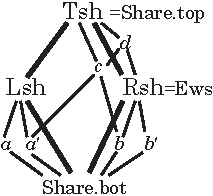
\includegraphics[scale=1.25]{graphics/shares.pdf}}

The \emph{top} share, written \lstinline{Tsh} or
\lstinline{Share.top}, gives total permission: to deallocate any cells
within the footprint of this mapsto, to read, to write.

\begin{lstlisting}
Share.split Tsh = (Lsh,Rsh)
Share.split Lsh = ($a,a'$)  $\qquad$ Share.split Rsh = ($b,b'$)
$a'\oplus b = c\qquad\qquad \mathrm{lub}(c,\mathsf{Rsh})=a'\oplus \mathsf{Rsh}=d$
\end{lstlisting}
Any share may be split into a \emph{left half} and a \emph{right half}.
The left and right of the top share are given distinguished names
\lstinline{Lsh, Rsh}.

The right-half share of the top share (or any share containing it such
as $d$) is sufficient to grant \emph{write permission} to the data:
``the right share is the write share.''  A thread of execution holding
only \lstinline{Lsh}---or subshares of it such as $a,a'$---can neither
read or write the object, but such shares are not completely useless:
holding any nonempty share prevents other threads from deallocating
the object.

Any subshare of \lstinline{Rsh}, in fact any share that overlaps
 \lstinline{Rsh}, grants \emph{read} permission to the object.
Overlap can be tested using the glb (greatest lower bound) operator.

Whenever \lstinline{(mapsto $\pi$ t v w)} holds, then the share $\pi$
must include at least a read share, thus this give permission to load
memory at address $v$ to get a value $w$ of type $t$.

To make sure $\pi$ has enough permission to write (i.e., 
$\mathsf{Rsh} \sqsubset \pi$, we can say \lstinline{writable_share $\pi$ : Prop}.

Memory obtained from \lstinline{malloc} comes with the top share
\lstinline{Tsh}.  Writable extern global variables
and stack-allocated addressable locals (which of course
must not be deallocated) come with the ``extern writable share'' 
\lstinline{Ews} which is equal to \lstinline{Rsh}.
Read-only globals come with a half-share of \lstinline{Rsh}.

Sequential programs usually have little need of any shares except
the \lstinline{Tsh} and \lstinline{Ews}.  However, many function 
specifications can be parameterized over any share, and this sort
of generalized specification makes the functions usable in more contexts.

In C it is undefined to test deallocated pointers for equality or inequalities,
so the Hoare-logic rule for pointer comparison also requires some
permission-share; see \autopageref{refcard:pointer-cmp}.


\ychapter{CompCert C}{}

The CompCert verified C compiler translates standard C source programs
into an abstract syntax for \emph{CompCert C},
and then translates that into abstract syntax
for \emph{C light}.  
Then VST Separation Logic is applied to the C light abstract syntax.
C light programs proved correct using the VST separation logic
can then be compiled (by CompCert) to assembly language.

C light syntax is defined by these Coq files from CompCert:

\begin{description}
\item[Integers.]  32-bit (and 8-bit, 16-bit, 64-bit) signed/unsigned integers.
\item[Floats.]  IEEE floating point numbers.
\item[Values.]  The \lstinline|val| type: integer + float + pointer + undefined.
\item[AST.]  Generic support for abstract syntax.
\item[Ctypes.]  C-language types and structure-field-offset computations.
\item[Cop.]  Semantics of C-language arithmetic operators.
\item[Clight.]  Abstract syntax of C-light expressions, statements, and functions.
\item[veric.expr.]  (from VST, not CompCert) Semantics of expression evaluation.
\end{description}

Some of the important types and operators are described over the next 
few pages.

\ychapter{Verifiable C programming}{See PLCC Chapter \ref{ch:compcert-intro}}
\label{refcard:verifiable-c}
In writing Verifiable C programs you must:

\begin{itemize}
  \item Make each dereference into a top level expression (PLCC
  \autopageref{verifiable-c})
  \item Make most pointer comparisons into a top level expression (PLCC
  \autopageref{pointercompare})
  \item Remove casts between \lstinline|int| and pointer types (result in
  values that crash if used)
\end{itemize}

The \lstinline{clightgen} tool automatically:

\begin{itemize}
  \item Factors function calls into top level expressions
  \item Factors logical \lstinline{and}/\lstinline{or} operators into 
\lstinline{if} statements (to capture
  short circuiting behavior)
\end{itemize}

Proof automation detects these two transformations and processes them with a
single tactic application.

If your program uses \lstinline|malloc| or \lstinline|free|, you must declare
and specify these as external functions. If you don't want to keep track of the
size of each allocated object, you may want to change the interface of the
\lstinline|free| function. We do this in our example definitions of
\lstinline|malloc| and \lstinline|free| in \file{progs/queue.c} and their
specifications in \file{progs/verif\_queue.v}.

\ychapter{32-bit Integers}{(\file{compcert/lib/Integers.v})}

The VST program logic uses CompCert's 32-bit integer type.

\begin{lstlisting}
Inductive comparison := Ceq | Cne | Clt | Cle | Cgt | Cge.
Definition wordsize: nat := 32.  (* also instantiations for 8, 16, 64 *)
Definition modulus : Z := two_power_nat wordsize.
Definition half_modulus : Z := modulus / 2.
Definition max_unsigned : Z := modulus - 1.
Definition max_signed : Z := half_modulus - 1.
Definition min_signed : Z := - half_modulus.

Parameter int : Type.
Parameter unsigned : int -> Z.
Parameter signed : int -> Z.
Parameter repr : Z -> int.

Definition zero := repr 0.

Definition eq (x y: int) : bool.
Definition lt (x y: int) : bool.
Definition ltu (x y: int) : bool.
Definition neg (x: int): int := repr (- unsigned x).
Definition add (x y: int): int :=  repr (unsigned x + unsigned y).
Definition sub (x y: int): int :=  repr (unsigned x - unsigned y).
Definition mul (x y: int): int :=  repr (unsigned x * unsigned y).
Definition divs (x y: int) : int.
Definition mods (x y: int) : int.
Definition divu (x y: int) : int.
Definition modu (x y: int) : int.
Definition and (x y: int): int := bitwise_binop andb x y.
Definition or (x y: int): int := bitwise_binop orb x y.
Definition xor (x y: int) : int := bitwise_binop xorb x y.
Definition not (x: int) : int := xor x mone.
Definition shl (x y: int): int.
Definition shru (x y: int): int.
Definition shr (x y: int): int.
Definition rol (x y: int) : int.
Definition ror (x y: int) : int.
Definition rolm (x a m: int): int.
Definition cmp (c: comparison) (x y: int) : bool.
Definition cmpu (c: comparison) (x y: int) : bool.

Lemma eq_dec: forall (x y: int), {x = y} + {x <> y}.
Theorem unsigned_range: forall i, 0 <= unsigned i < modulus.
Theorem unsigned_range_2:  forall i, 0 <= unsigned i <= max_unsigned.
Theorem signed_range:  forall i, min_signed <= signed i <= max_signed.
Theorem repr_unsigned:  forall i, repr (unsigned i) = i.
Lemma repr_signed:  forall i, repr (signed i) = i.
Theorem unsigned_repr: 
   forall z, 0 <= z <= max_unsigned -> unsigned (repr z) = z.
Theorem signed_repr:
  forall z, min_signed <= z <= max_signed -> signed (repr z) = z.
Theorem signed_eq_unsigned:
  forall x, unsigned x <= max_signed -> signed x = unsigned x.

Theorem unsigned_zero: unsigned zero = 0.
Theorem unsigned_one: unsigned one = 1.
Theorem signed_zero: signed zero = 0.

Theorem eq_sym:  forall x y, eq x y = eq y x.
Theorem eq_spec: forall (x y: int), if eq x y then x = y else x <> y.
Theorem eq_true: forall x, eq x x = true.
Theorem eq_false: forall x y, x <> y -> eq x y = false.

Theorem add_unsigned: forall x y, add x y = repr (unsigned x + unsigned y).
Theorem add_signed: forall x y, add x y = repr (signed x + signed y).
Theorem add_commut: forall x y, add x y = add y x.
Theorem add_zero: forall x, add x zero = x.
Theorem add_zero_l: forall x, add zero x = x.
Theorem add_assoc: forall x y z, add (add x y) z = add x (add y z).

Theorem neg_repr: forall z, neg (repr z) = repr (-z).
Theorem neg_zero: neg zero = zero.
Theorem neg_involutive: forall x, neg (neg x) = x.
Theorem neg_add_distr: forall x y, neg(add x y) = add (neg x) (neg y).

Theorem sub_zero_l: forall x, sub x zero = x.
Theorem sub_zero_r: forall x, sub zero x = neg x.
Theorem sub_add_opp: forall x y, sub x y = add x (neg y).
Theorem sub_idem: forall x, sub x x = zero.
Theorem sub_add_l: forall x y z, sub (add x y) z = add (sub x z) y.
Theorem sub_add_r: forall x y z, sub x (add y z) = add (sub x z) (neg y).
Theorem sub_shifted: forall x y z, sub (add x z) (add y z) = sub x y.
Theorem sub_signed:  forall x y, sub x y = repr (signed x - signed y).

Theorem mul_commut: forall x y, mul x y = mul y x.
Theorem mul_zero: forall x, mul x zero = zero.
Theorem mul_one: forall x, mul x one = x.
Theorem mul_assoc: forall x y z, mul (mul x y) z = mul x (mul y z).
Theorem mul_add_distr_l: forall x y z, mul (add x y) z = add (mul x z) (mul y z).
Theorem mul_signed: forall x y, mul x y = repr (signed x * signed y).
\end{lstlisting}
and many more axioms for the bitwise operators, shift operators,
signed/unsigned division and mod operators.


\ychapter{Values}{(\file{compcert/common/Values.v})}

\begin{lstlisting}
Definition block : Type := positive.

Inductive val: Type :=
  | Vundef: val
  | Vint: int -> val
  | Vlong: int64 -> val
  | Vfloat: float -> val
  | Vptr: block -> int -> val.
\end{lstlisting}

\lstinline{Vundef} is the \emph{undefined} value---found, for example,
in an uninitialized local variable.

\lstinline{Vint($i$)} is an integer value,
where $i$ is a CompCert 32-bit integer.

\lstinline{Vfloat($f$)} is an floating-point value,
where $f$ is a Flocq 64-bit floating-point number.

\lstinline{Vptr $b$ $z$} is a pointer value,
where $b$ is an abstract block number and $z$ is an offset
within that block.  Different \emph{malloc} operations,
or different extern global variables, or 
stack-memory-resident local variables,
will have different abstract block numbers.
Pointer arithmetic must be done within the same abstract block,
with $(\mathsf{Vptr}\,b\,z)+(\mathsf{Vint}~i)~=~\mathsf{Vptr}\,b\,(z+i)$.
Of course, the C-language + operator first multiplies $i$
by the size of the array-element that 
$\mathsf{Vptr}\,b\,z$ points to.

\ychapter{C types}{(\file{compcert/cfrontend/Ctypes.v})}
\begin{lstlisting}
Inductive signedness := Signed | Unsigned.
Inductive intsize := I8 | I16 | I32 | IBool.
Inductive floatsize :=  F32 | F64.

Record attr : Type := mk_attr {
  attr_volatile: bool
}.
Definition noattr := {| attr_volatile := false |}.

Inductive type : Type :=
  | Tvoid: type                                
  | Tint: intsize -> signedness -> attr -> type
  | Tlong: signedness -> attr -> type
  | Tfloat: floatsize -> attr -> type          
  | Tpointer: type -> attr -> type             
  | Tarray: type -> Z -> attr -> type          
  | Tfunction: typelist -> type -> type        
  | Tstruct: ident -> fieldlist -> attr -> type
  | Tunion: ident -> fieldlist -> attr -> type 
  | Tcomp_ptr: ident -> attr -> type           

with typelist : Type :=
  | Tnil: typelist
  | Tcons: type -> typelist -> typelist

with fieldlist : Type :=
  | Fnil: fieldlist
  | Fcons: ident -> type -> fieldlist -> fieldlist.

Definition typeconv (ty: type) : type :=
  match ty with
  | Tint (I8 | I16 | IBool) _ a => Tint I32 Signed a
  | Tarray t sz a       => Tpointer t a
  | Tfunction _ _       => Tpointer ty noattr
  | _                   => ty
  end.

Fixpoint alignof (t: type) : Z :=
  match t with
  | Tint I8 _ _ => 1
  | Tint I16 _ _ => 2
  | Tint I32 _ _ => 4
  | Tlong _ _ => 8
  | Tfloat F32 _ => 4
  | Tfloat F64 _ => 8
  | Tpointer _ _ => 4
  ... $et~cetera$
  end.

(** Size of a type, in bytes. *)

Fixpoint sizeof (t: type) : Z :=
  match t with
  | Tint I8 _ _ => 1
  | Tint I16 _ _ => 2
  | Tint I32 _ _ => 4
  | Tlong _ _ => 8
  | Tfloat F32 _ => 4
  | Tfloat F64 _ => 8
  | Tpointer _ _ => 4
  ... $et~cetera$
  end.

Lemma sizeof_pos:  forall t, sizeof t > 0.


Definition field_offset (id: ident) (fld: fieldlist) : res Z.

Fixpoint field_type (id: ident) (fld: fieldlist) {struct fld} : res type.

Inductive mode: Type :=
  | By_value: memory_chunk -> mode
  | By_reference: mode
  | By_copy: mode
  | By_nothing: mode.

Definition access_mode (ty: type) : mode :=
  match ty with
  | Tint I8 Signed _ => By_value Mint8signed
  | Tint I8 Unsigned _ => By_value Mint8unsigned
  | Tint I16 Signed _ => By_value Mint16signed
  | Tint I16 Unsigned _ => By_value Mint16unsigned
  | Tint I32 _ _ => By_value Mint32
  | Tint IBool _ _ => By_value Mint8unsigned
  | Tlong _ _ => By_value Mint64
  | Tfloat F32 _ => By_value Mfloat32
  | Tfloat F64 _ => By_value Mfloat64
  | Tvoid => By_nothing
  | Tpointer _ _ => By_value Mint32
  | Tarray _ _ _ => By_reference
  | Tfunction _ _ => By_reference
  | Tstruct _ _ _ => By_copy
  | Tunion _ _ _ => By_copy
  | Tcomp_ptr _ _ => By_nothing
end.
\end{lstlisting}

\clearpage
\newthought{CompCert} handles self-referential structure types
in the following way that deserves at least some explanation,
not provided here:
\begin{lstlisting}
Fixpoint unroll_composite (cid: ident) (comp: type) (ty: type) : type :=
  match ty with
  | Tvoid => ty
  | Tint _ _ _ => ty
  | Tlong _ _ => ty
  | Tfloat _ _ => ty
  | Tpointer t1 a => Tpointer (unroll_composite t1) a
  | Tarray t1 sz a => Tarray (unroll_composite t1) sz a
  | Tfunction t1 t2 => 
        Tfunction (unroll_composite_list t1) (unroll_composite t2)
  | Tstruct id fld a => 
        if ident_eq id cid then ty 
        else Tstruct id (unroll_composite_fields fld) a
  | Tunion id fld a => 
        if ident_eq id cid then ty 
        else Tunion id (unroll_composite_fields fld) a
  | Tcomp_ptr id a => 
        if ident_eq id cid then Tpointer comp a else ty
  end

with unroll_composite_list cid comp(tl: typelist) : typelist := ...
with unroll_composite_fields cid comp (fld: fieldlist) : fieldlist := ...

Lemma alignof_unroll_composite:
  forall cid comp ty, alignof (unroll_composite cid comp ty) = alignof ty.

Lemma sizeof_unroll_composite:
  forall cid comp ty, sizeof (unroll_composite cid comp ty) = sizeof ty.
\end{lstlisting}
\ychapter{C expression syntax}{(\file{compcert/cfrontend/Clight.v})}

\begin{lstlisting}
Inductive expr : Type :=
(* 1$~$  *) $~~~$   | Econst_int: int -> type -> expr      
(* 1.0 *)   $~$ | Econst_float: float -> type -> expr  (* double precision *)
(* 1.0f0 *)    | Econst_single: float -> type -> expr (* single precision *)
(* 1L  *)  $~~$  | Econst_long: int64 -> type -> expr
(* x   *) $~~~~$   | Evar: ident -> type -> expr         
(* x   *) $~~~~$   | Etempvar: ident -> type -> expr     
(* *e  *) $~~~$   | Ederef: expr -> type -> expr        
(* &e  *) $~~$   | Eaddrof: expr -> type -> expr       
(* ~e  *) $~~$   | Eunop: unary_operation -> expr -> type -> expr
(* e+e *) $~$   | Ebinop: binary_operation -> expr -> expr -> type -> expr 
(* (int)e *) | Ecast: expr -> type -> expr  
(* e.f *) $~~$ | Efield: expr -> ident -> type -> expr. 

Definition typeof (e: expr) : type :=
  match e with
  | Econst_int _ ty => ty
  | Econst_float _ ty => ty
  | Evar _ ty => ty
  | ... $et~cetera$.
\end{lstlisting}

\ychapter{C operators}{(\file{compcert/cfrontend/Cop.v})}
\begin{lstlisting}

Function bool_val (v: val) (t: type) : option bool :=
  match classify_bool t with
  | bool_case_i =>
      match v with
      | Vint n => Some (negb (Int.eq n Int.zero))
      | _ => None
      end
  | bool_case_f =>
      match v with
      | Vfloat f => Some (negb (Float.cmp Ceq f Float.zero))
      | _ => None
      end
  | bool_case_p =>
      match v with
      | Vint n => Some (negb (Int.eq n Int.zero))
      | Vptr b ofs => Some true
      | _ => None
      end
  | bool_default => None
  end.

Function sem_neg (v: val) (ty: type) : option val :=
  match classify_neg ty with
  | neg_case_i sg =>
      match v with
      | Vint n => Some (Vint (Int.neg n))
      | _ => None
      end
  | neg_case_f =>
      match v with
      | Vfloat f => Some (Vfloat (Float.neg f))
      | _ => None
      end
  | neg_default => None
  end.

Function sem_add (v1:val) (t1:type) (v2: val) (t2:type) : option val :=
  match classify_add t1 t2 with 
  | add_case_ii sg =>                   (**r integer addition *)
      match v1, v2 with
      | Vint n1, Vint n2 => Some (Vint (Int.add n1 n2))
      | _,  _ => None
      end
  | add_case_ff =>                      (**r float addition *)
      match v1, v2 with
      | Vfloat n1, Vfloat n2 => Some (Vfloat (Float.add n1 n2))
      | _,  _ => None
      end
  | add_case_if sg =>                   (**r int plus float *)
      match v1, v2 with
      | Vint n1, Vfloat n2 => Some (Vfloat (Float.add (cast_int_float sg n1) n2))
      | _, _ => None
      end
  | ... $(cases~omitted)$
  | add_case_ip ty _ =>                 (**r integer plus pointer *)
      match v1,v2 with
      | Vint n1, Vptr b2 ofs2 => 
        Some (Vptr b2 (Int.add ofs2 (Int.mul (Int.repr (sizeof ty)) n1)))
      | _,  _ => None
      end   
  | add_default => None
end.

Function sem_sub (v1:val) (t1:type) (v2: val) (t2:type) : option val.
Function sem_mul (v1:val) (t1:type) (v2: val) (t2:type) : option val.
Function sem_div (v1:val) (t1:type) (v2: val) (t2:type) : option val.
Function sem_mod (v1:val) (t1:type) (v2: val) (t2:type) : option val.
Function sem_and (v1:val) (t1:type) (v2: val) (t2:type) : option val.

Function sem_cmp (c:comparison)
                  (v1: val) (t1: type) (v2: val) (t2: type)
                  (m: mem): option val :=
  match classify_cmp t1 t2 with
  | cmp_case_ii Signed =>
      match v1,v2 with
      | Vint n1, Vint n2 => Some (Val.of_bool (Int.cmp c n1 n2))
      | _,  _ => None
      end
  | ... $(many~more~cases~)$
  end.

Definition sem_binary_operation
    (op: binary_operation)
    (v1: val) (t1: type) (v2: val) (t2:type)
    (m: mem): option val :=
  match op with
  | Oadd => sem_add v1 t1 v2 t2
  | Osub => sem_sub v1 t1 v2 t2 
  | Omul => sem_mul v1 t1 v2 t2
  | Omod => sem_mod v1 t1 v2 t2
  | Odiv => sem_div v1 t1 v2 t2 
  | Oand => sem_and v1 t1 v2 t2
  | Oor  => sem_or v1 t1 v2 t2
  | Oxor  => sem_xor v1 t1 v2 t2
  | Oshl => sem_shl v1 t1 v2 t2
  | Oshr  => sem_shr v1 t1 v2 t2   
  | Oeq => sem_cmp Ceq v1 t1 v2 t2 m
  | One => sem_cmp Cne v1 t1 v2 t2 m
  | Olt => sem_cmp Clt v1 t1 v2 t2 m
  | Ogt => sem_cmp Cgt v1 t1 v2 t2 m
  | Ole => sem_cmp Cle v1 t1 v2 t2 m
  | Oge => sem_cmp Cge v1 t1 v2 t2 m
  end.
\end{lstlisting}

\ychapter{C expression evaluation}{(\file{vst/veric/expr.v})}

\begin{lstlisting}
Definition eval_id (id: ident) ($\rho$: environ).
  (* look up the tempory variable ``id'' in $\rho$ *)

Definition eval_cast (t t': type) (v: val) : val.
  (* cast value v from type t to type t', but beware! There are
     be $three$ types involved, if you include the native type of v. *)

Definition eval_unop (op: Cop.unary_operation) (t1 : type) (v1 : val) : val.

Definition eval_binop (op: Cop.binary_operation) 
               (t1 t2 : type) (v1 v2: val) : val.

Definition force_ptr (v: val) : val :=
       match v with Vptr l ofs => v | _ => Vundef  end.

Definition eval_struct_field (delta: Z) (v: val) : val.
   (* offset the pointer-value v by delta *)

Definition eval_field (ty: type) (fld: ident) (v: val) : val.
   (* calculate the lvalue of (but do not fetch/dereference!)
      a structure/union field of value v *)

Definition eval_var (id:ident) (ty: type) (rho: environ) : val.
   (* Get the lvalue (address of) an addressable local variable
     (if there is one of that name) or else a global variable *)

Definition deref_noload (ty: type) (v: val) : val.
   (* For By_reference types such as arrays that dereference
      without actually fetching *)
 match access_mode ty with By_reference => v | _ => Vundef end.
\end{lstlisting}

\clearpage
\begin{lstlisting}
Fixpoint eval_expr (e: expr) : environ -> val :=
 match e with
 | Econst_int i ty => `(Vint i)
 | Econst_float f ty => `(Vfloat f)
 | Etempvar id ty => eval_id id 
 | Eaddrof a ty => eval_lvalue a 
 | Eunop op a ty =>  `(eval_unop op (typeof a)) (eval_expr a) 
 | Ebinop op a1 a2 ty =>  
           `(eval_binop op (typeof a1) (typeof a2))
              (eval_expr a1) (eval_expr a2)
 | Ecast a ty => `(eval_cast (typeof a) ty) (eval_expr a) 
 | Evar id ty => `(deref_noload ty) (eval_var id ty)
 | Ederef a ty => `(deref_noload ty) (`force_ptr (eval_expr a))
 | Efield a i ty => `(deref_noload ty) 
                      (`(eval_field (typeof a) i) (eval_lvalue a))
 end

 with eval_lvalue (e: expr) : environ -> val := 
 match e with 
 | Evar id ty => eval_var id ty
 | Ederef a ty => `force_ptr (eval_expr a)
 | Efield a i ty => `(eval_field (typeof a) i) (eval_lvalue a)
 | _  => `Vundef
 end.
\end{lstlisting}

\ychapter{C type checking}{(See PLCC \autoref{ch:typecheck})}
Ideally, you will never notice the typechecker, but it may occasionally
generate side conditions that can not be solved automatically.
If you get a proof goal from the typechecker, it will be an entailment 
\lstinline!P |-- denote_tc_assert ($\ldots$)!. PLCC
\autoref{ch:clight-auto} discusses what you can do to solve these goals. 

If you are asked to prove an entailment where the typechecking condition
evaluates to \lstinline|False|, this may be because your program is not written in
Verifiable C. You may need to perform some local transformations on your C
program in order to proceed. We listed these transformations on
\autopageref{refcard:verifiable-c}. 

The type-context will always be visible in your proof in a line that looks like 
\lstinline|Delta := abbreviate : tycontext|. The \lstinline|abbreviate|
hides the implementation of the type context (which is generally large
and uninteresting). The
\lstinline|query_context| tactic shows the result of looking up a variable in
a typecontext. The tactic \lstinline|query_context Delta _p.| will add hypothesis
\lstinline|QUERY : (temp_types Delta) ! _p = Some (tptr t_struct_list, true)|.
This means that in \lstinline|Delta|, \lstinline|_p| is a temporary variable
with type \lstinline|tptr t_struct_list| and that it is known to be initialized.

\ychapter{Lifted separation logic}{(See PLCC \autoref{ch:lifted})}
Assertions in our Hoare triple of separation 
are presented as $\mathsf{env}\rightarrow
\mathsf{mpred}$, that is, functions from environment
to memory-predicate,
using our natural deduction system 
\lstinline{NatDed(mpred)} and separation logic
\lstinline{SepLog(mpred)}.

Given a separation logic over a type $B$ of formulas,
and an arbitrary type $A$, 
we can define a \emph{lifted} separation logic over functions $A \rightarrow B$.
The operations are simply lifted pointwise over the
elements of $A$.  Let $P,Q:~A\rightarrow B$,
let $R:T\rightarrow A \rightarrow B$ then define,
\[
\begin{array}{rccl}
(P \andp Q):& A\rightarrow B&:=& \mathrm{fun}~a~\Rightarrow~Pa \andp Qa\\
(P \orp Q):& A\rightarrow B&:=& \mathrm{fun}~a~\Rightarrow~Pa \orp Qa\\
(\exists x.R(x)):& A\rightarrow B&:=& \mathrm{fun}~a~\Rightarrow~\exists x.~Rxa\\
(\forall x.R(x)):& A\rightarrow B&:=& \mathrm{fun}~a~\Rightarrow~\forall x.~Rxa\\
(P \imp Q):& A\rightarrow B&:=& \mathrm{fun}~a~\Rightarrow~Pa \imp Qa\\
(P \vdash Q):& A\rightarrow B&:=& \forall a.~Pa \vdash Qa\\
(P * Q):& A\rightarrow B&:=& \mathrm{fun}~a~\Rightarrow~Pa * Qa\\
(P \wand Q):& A\rightarrow B&:=& \mathrm{fun}~a~\Rightarrow~Pa \wand Qa\\
\end{array}
\]
In Coq we formalize the typeclass instances
\lstinline{LiftNatDed},
\lstinline{LiftSepLog}, etc.,
as shown below.
For a type $B$, whenever \lstinline{NatDed B} and \lstinline{SepLog B} (and so on) have been defined, the lifted instances
\lstinline{NatDed (A->B)} and \lstinline{SepLog (A->B)} (and so on)
are automagically provided by the typeclass system.

\begin{lstlisting}
Instance LiftNatDed(A B: Type){ND: NatDed B}: NatDed (A->B):=
 mkNatDed (A -> B)
    (*andp*) (fun P Q x => andp (P x) (Q x))
    (*orp*) (fun P Q x => orp (P x) (Q x))
    (*exp*) (fun {T} (F: T -> A -> B) (a: A) => exp (fun x => F x a))
    (*allp*) (fun {T} (F: T -> A -> B) (a: A) => allp (fun x => F x a))
    (*imp*) (fun P Q x => imp (P x) (Q x))
    (*prop*) (fun P x => prop P)
    (*derives*) (fun P Q => forall x, derives (P x) (Q x))
     _ $$ _ $$ _ $$ _ $$ _ $$ _ $$ _ $$ _ $$ _ $$ _ $$ _ $$ _ $$ _ $$ _ $$ _ $$ _ $$ _ $$ _.

Instance LiftSepLog (A B: Type) {NB: NatDed B}{SB: SepLog B} 
      : SepLog (A -> B).
 apply (mkSepLog (A -> B) _ (fun $\rho$ => emp) 
            (fun P Q $\rho$ => P $\rho$ * Q $\rho$) (fun P Q $\rho$ => P $\rho$ -* Q $\rho$)).
 (* fill in proofs here *)
\end{lstlisting}

In particular, if $P$ and $Q$ are functions of type \lstinline{environ->mpred}
then we can write $P*Q$,  $P \andp Q$, and so on.

Consider this assertion:
\begin{lstlisting}
fun $\rho$ => mapsto $\pi$ tint (eval_id _x $\rho$) (eval_id _y $\rho$) 
             * mapsto $\pi$ tint (eval_id _u $\rho$) (Vint Int.zero)
\end{lstlisting}
which might appear as the precondition of a Hoare triple.
It represents $(x\mapsto y) *(u\mapsto 0)$ written in informal
separation logic, where $x,y,u$ are C-language variables
of integer type.
Because it can be inconvenient to manipulate explicit lambda expressions
and explicit environment variables $\rho$, we may write it in lifted
form,
\begin{lstlisting}
 `(mapsto $\pi$ tint) (eval_id _x) (eval_id _y) 
* `(mapsto $\pi$ tint) (eval_id _u) `(Vint Int.zero)
\end{lstlisting}
Each of the first two backquotes lifts a function
from type \lstinline{val->val->mpred} to type
\lstinline{(environ->val)->(environ->val)->(environ->mpred)},
and the third one lifts from \lstinline{val} to 
\lstinline{environ->val}.

\ychapter{Canonical forms}{(See PLCC \autoref{canonical-form})}
We write a \emph{canonical form} of an assertion as,
\[
\PROP(P_0;P_1;\ldots,P_{l-1})~
\LOCAL(Q_0;Q_1;\ldots,Q_{m-1})~
\SEP(R_0;R_1;\ldots,R_{n-1})
\]
The $P_i : \mathsf{Prop}$ are Coq propositions---these are independent
of the program variables and the memory.
The $Q_i : \mathsf{environ}->\mathsf{Prop}$ are local---they depend on 
program variables but not on memory.
The $R_i: \mathsf{environ}->\mathsf{mpred}$ are 
assertions of separation logic,
which may depend on both program variables and memory.

The $\PROP/\LOCAL/\SEP$ form is defined formally as,
\begin{lstlisting}
Definition PROPx (P: list Prop) (Q: assert) := 
          andp (prop (fold_right and True P)) Q.
Notation "'PROP' ( x ; .. ; y )   z" := 
      (PROPx (cons x%type .. (cons y%type nil) ..) z) (at level 10) : logic.
Notation "'PROP' ( )   z" :=   (PROPx nil z) (at level 10) : logic.

Definition LOCALx (Q: list (environ -> Prop)) (R: assert) := 
                 andp (local (fold_right (`and) (`True) Q)) R.
Notation " 'LOCAL' ( x ; .. ; y )   z" := 
     (LOCALx (cons x%type .. (cons y%type nil) ..) z) (at level 9) : logic.
Notation " 'LOCAL' ( )   z" := (LOCALx nil z)  (at level 9) : logic.

Definition SEPx (R: list assert) : assert := fold_right sepcon emp R.

Notation " 'SEP' ( x ; .. ; y )" := 
        (SEPx (cons x%logic .. (cons y%logic nil) ..)) (at level 8) : logic.
Notation " 'SEP' ( ) " := (SEPx nil) (at level 8) : logic.
Notation " 'SEP' () " := (SEPx nil) (at level 8) : logic.
\end{lstlisting}
Thus, 
$\PROP (P_0;P_1)\,\LOCAL(Q_0;Q_1)\,\SEP\,(R_0;R_1)$
is equivalent to 
$\mathsf{prop}\,P_0\wedge \mathsf{prop}\,P_1 \andp
\mbox{\textbf{\`{}}}\mathsf{prop}\,Q_0 \andp \mbox{\textbf{\`{}}}\mathsf{prop}\,Q_1 \andp
(R_0 * R_1)$.

\ychapter{Supercanonical forms}{}
\label{refcard:supercanonical}

A canonical form \(\PROP (\vec{P})\,\LOCAL(\vec{Q})\,\SEP\,(\vec{R})\)
is \emph{supercanonical} if:
\begin{itemize}
\item Every element of $\vec{Q}$ has the form
~~\lstinline{temp $i$ $V$}~
or ~~\lstinline{var $i$ $t$ $V$},\newline
where $V$ is a Coq expression of type \lstinline{val}
and $i$ is $\beta\eta$-equivalent to 
a constant (a ground term of type \lstinline{ident}).
The term ~\lstinline{temp $i$ $V$}
(of type \lstinline{environ->Prop})
is equivalent to 
\lstinline{`(eq $V$) (eval_id $i$)}.
The term ~\lstinline{var $i$ $t$ $V$}
(of type \lstinline{environ->Prop})
is equivalent to 
\lstinline{`(eq $V$) (eval_var $i$ $t$)}.

\item Every element of $R$ is
~\lstinline{`($E$)} where $E$ is a Coq expression of type \lstinline{mpred}.
\end{itemize}

When assertions (preconditions of \lstinline{semax}) are kept
in supercanonical form, the \lstinline{forward} tactic
for symbolic execution runs \emph{much} faster.  That is,
\begin{itemize}
\item \lstinline{forward} through assignment statements
(including loads/stores) is up to 10 times faster for supercanonical
preconditions than for ordinary (canonical) preconditions.
\item Future versions of the forward tactic may \emph{require}
the precondition to be in supercanonical form.
\end{itemize}

\ychapter{Go\_lower}{(See PLCC \autoref{ch:clight-auto})}
\label{refcard:go-lower}
An entailment 
$\PROP (\vec{P})\,\LOCAL(\vec{Q})\,\SEP\,(\vec{R})~
\vdash ~
\PROP (\vec{P'})\,\LOCAL(\vec{Q'})\,\SEP\,(\vec{R'})
$
is a sequent in our \emph{lifted} separation logic;
each side
has type \lstinline{environ->mpred}.  By definition of the lifted
entailment $\vdash$ it means exactly,\linebreak
$\forall \rho.~
\PROP (\vec{P})\,\LOCAL(\vec{Q})\,\SEP\,(\vec{R})\,\rho
\vdash 
\PROP (\vec{P'})\,\LOCAL(\vec{Q'})\,\SEP\,(\vec{R'})\,\rho
$. \linebreak
There are two ways to prove such an entailment:
Explicitly introduce $\rho$ (descend
into an entailment on \lstinline{mpred}) and 
unfold the $\PROP/\LOCAL/\SEP$ form; 
or stay in canonical form and rewrite in
the lifted logic.
Either way may be appropriate; this chapter describes
how to descend.
The \lstinline{go_lower} tactic, described on this page,
is rarely called directly; it is the first step of the
\lstinline{entailer} tactic (\autopageref{refcard:entailer})
when applied to lifted entailments.

The tactic \lstinline{go_lower} tactic
does the following:
\begin{enumerate}
\item \lstinline{intros ?rho}, as described above.
\item If the first conjunct of the 
left-hand-side \textsc{local}s is
\lstinline{tc_environ $\Delta$ $\rho$}, move it
above the line; this be useful in step \ref{step-findvars}.
\item Unfold definitions for
\emph{canonical forms}
(\lstinline{PROPx LOCALx SEPx}),
\emph{expression evaluation}
(\lstinline{eval_exprlist}
\lstinline{eval_expr}
\lstinline{eval_lvalue}
\lstinline{cast_expropt}
\lstinline{eval_cast}
\lstinline{eval_binop}
\lstinline{eval_unop}),
\emph{casting} (\lstinline{eval_cast} \lstinline{classify_cast})
\emph{typechecking} (\lstinline{tc_expropt}
\lstinline{tc_expr}
\lstinline{tc_lvalue}
\lstinline{typecheck_expr}
\lstinline{typecheck_lvalue}
\lstinline{denote_tc_assert}),
\emph{function postcondition operators} (\lstinline{function_body_ret_assert}
\lstinline{make_args'}
\lstinline{bind_ret}
\lstinline{get_result1}
\lstinline{retval}),
\emph{lifting operators} (\lstinline{liftx}
\lstinline{LiftEnviron}
\lstinline{Tarrow}
\lstinline{Tend}
\lstinline{lift_S}
\lstinline{lift_T}
\lstinline{lift_prod}
\lstinline{lift_last}
\lstinline{lifted}
\lstinline{lift_uncurry_open}
\lstinline{lift_curry}
\lstinline{local}
\lstinline{lift}
\lstinline{lift0}
\lstinline{lift1}
\lstinline{lift2}
\lstinline{lift3}).
\item Simplify by \lstinline{simpl}.
\item Rewrite by the rewrite-hint environment \lstinline{go_lower}, which contains just a very few rules to evaluate certain environment lookups.
\item Recognize local variables. \label{step-findvars}
\end{enumerate}

Local variables that appear in the lifted canonical form
as \lstinline{(eval_id _x)} will be replaced by
Coq variables \lstinline{x}, provided that:
(1)  $\vec{Q}$ includes a clause of the
form \lstinline{(tc_environ $\Delta$)},
and (2) there is a hypothesis \lstinline{name x _x} ``above the line.''
(See PLCC \autoref{go-lower-findvars}).
In addition, a typechecking hypothesis for \lstinline{x}
will be introduced above the line (see \autoref{refcard:tcval}).

\ychapter{Welltypedness of variables}{}
\label{refcard:tcval}

The typechecker ensures some invariants about the values
of C-program variables: if a variable is initialized, it contains
a value of its declared type.

Function parameters (accessed by
\lstinline{Etempvar} expressions)
are always initialized.
Nonaddressable local variables (accessed by
\lstinline{Etempvar} expressions) and address-taken local variables
(accessed by \lstinline{Evar})
may be uninitialized or initialized. 
Global variables (accessed by \lstinline{Evar}) are always
initialized.

The typechecker keeps track of the
initialization status of local nonaddressable 
variables, \emph{conservatively:}
if on all paths from function entry to the current
point---assuming that the conditions on if-expressions
and while-expressions are uninterpreted/nondeterministic---there
is an assignment to variable $x$, then $x$ is known to
be initialized.

The initialization status of addressable local variables
is tracked in the separation logic,
by assertions such as $v \mapsto \_$
or $v \mapsto i$ for uninitialized and initialized variables,
respectively.

Proofs using the \lstinline{forward} tactic will typically
generate proof obligations (for the user to solve)
of the form,
\[
\PROP(\vec{P})~
\LOCAL(\mathsf{tc\_environ}\,\Delta; \vec{Q})~
\SEP(\vec{R})
~\vdash
\PROP(\vec{P'})~
\LOCAL(\vec{Q'})~
\SEP(\vec{R'})
\]

The conjunct (\lstinline{tc_environ $\Delta$})
keeps track of which nonaddressable local variables are initialized;
says that all references to local variables
contain values of the right type;
and says that all addressable locals and globals point
to an appropriate block of memory.

The \lstinline{go_lower} tactic
(usually) deletes the assertion 
\lstinline{tc_environ $\Delta$ $\rho$}
after deriving type-checking assertions of the form
\lstinline{tc_val $\tau$ v}
for each variable $v$ of type $\tau$;
it puts these assertions above the line.
\pagebreak
\begin{lstlisting}
Definition tc_val ($\tau$: type) : val -> Prop :=
 match $\tau$ with 
 | Tint sz sg _ $$ => is_int sz sg
 | Tlong _ $$ _ $$ => is_long 
 | Tfloat F64 _ $$ => is_float
 | Tfloat F32 _ $$ => is_single
 | Tpointer _ $$ _ $$ | Tarray _ $$ _ $$ _ $$ 
   | Tfunction _ $$ _ $$ _ $$ | Tcomp_ptr _ $$ _ $$ => is_pointer_or_null
 | Tstruct _ $$ _ $$ _ $$ => isptr
 | Tunion _ $$ _ $$ _ $$ => isptr
 | _ $$ => (fun _ $$ => False)
 end.
\end{lstlisting}
Since $\tau$ is concrete, \lstinline{tc_val $\tau$ v}
immediately unfolds
to something like,
\begin{lstlisting}
TC0: is_int I32 Signed (Vint i)
TC1: is_int I8 Unsigned (Vint c)
TC2: is_int I8 Signed (Vint d)
TC3: is_pointer_or_null p
TC4: isptr q
\end{lstlisting}

\lstinline{TC0} says that $i$ is a 32-bit signed integer;
this is a tautology, so it will be automatically deleted by
\lstinline{go_lower}.

\lstinline{TC1} says that $c$ is a 32-bit signed integer
whose value is in the range of unsigned 8-bit integers
(unsigned char).
\lstinline{TC2} says that $d$ is a 32-bit signed integer
whose value is in the range of signed 8-bit integers
(signed char).
These hypotheses simplify to,
\begin{lstlisting}
TC1: 0 <= Int.unsigned c <= Byte.max_unsigned
TC2: Byte.min_signed <= Int.signed c <= Byte.max_signed
\end{lstlisting}

\chapter{Normalize}
The \lstinline{normalize} tactic performs
\lstinline{autorewrite with norm} and several other transformations.
Many of the simplifications performed by \lstinline{normalize}
on entailments (whether lifted or unlifted)
can be done more efficiently and systematically by
\lstinline{entailer}.  However, on Hoare triples, \lstinline{entailer}
does not apply, and \lstinline{normalize} is quite appropriate.

The \lstinline{norm} rewrite-hint database uses several sets of rules.

\textbf{Generic separation-logic simplifications.}
\begin{mathpar}
P*\mathsf{emp}=P \and 
\mathsf{emp}*P=P \and 
P \andp  \TT = P \and
\TT \andp  P = P \and
(EX x:A,P)*Q = EX x:A,P*Q\and
P*(EX x:A,Q) = EX x:A,P*Q\and
(EX x:A,P)\andp Q = EX x:A,P\andp Q\and
P\andp (EX x:A,Q) = EX x:A,P\andp Q\and
P*(!!Q\andp R)=!!Q\andp (P*R) \and 
(!!Q\andp P)*R=!!Q\andp (P*R) \and 
P \andp  \FF = \FF \and
\FF \andp  P = \FF \and
P *  \FF = \FF \and
\FF *  P = \FF \and
P \rightarrow (!!P \andp Q = Q) \and
P \rightarrow (!!P = \TT) \and
P \andp P = P \and
(\mathsf{EX} \_:\_,P)=P \and 
\mathsf{local}~`\mathsf{True}=\TT 
\end{mathpar}

\textbf{Unlifting.}
\begin{mathpar}
`f~\rho~= f~\mbox{\small [when f has arity 0]}\and
`f~a_1~\rho~= f~(a_1~\rho)~\mbox{\small [when f has arity 1]}\and
`f~a_1~a_2~\rho~= f~(a_1~\rho)~(a_2~\rho)~\mbox{\small [when f has arity 2, etc.]}\and
\mathsf{local}~P~\rho = !!(P~\rho) \and
(P*Q)\rho = P\rho*Q\rho \and
(P\andp Q)\rho = P\rho\andp Q\rho \and
(!!P)\rho = !!P \and
!!(P\wedge Q) = !!P \andp !!Q \and
(\mathsf{EX}\,x:A,\,P\,x)\,\rho~=~\mathsf{EX}\,x:A,\,~P\,x\,\rho \and
`(\mathsf{EX}~x:B,~P x)= \mathsf{EX}~x:B,~`(P x)) \and
`(P*Q)=~`P\,*\,`Q \and
`(P\andp Q)=~`P\,\andp\,`Q 
\end{mathpar}

\textbf{Pulling nonspatial propositions out of spatial ones.}
\begin{mathpar}
\mathsf{local}~P~\andp~!!Q =
!!Q~\andp~\mathsf{local}~P \and
\mathsf{local}~P~\andp~(!!Q\andp R) =
!!Q\andp (\mathsf{local}~P~\andp~R) \and
(\mathsf{local}~P~\andp~Q)* R =
\mathsf{local}~P~\andp~(Q* R) \and
Q*(\mathsf{local}~P~\andp~ R) =
\mathsf{local}~P~\andp~(Q* R) 
\end{mathpar}

\textbf{Canonical forms.}
\begin{mathpar}
\mathsf{local}~Q_1\andp(\PROP(\vec{P} )\LOCAL(\vec{Q})\SEP(\vec{R}))=
\PROP(\vec{P})\LOCAL(Q_1;\vec{Q}) \SEP (\vec{R})\and
\PROP \vec{P} \LOCAL \vec{Q} \SEP (!!P_1; \vec{R})=
\PROP (P_1;\vec{P}) \LOCAL (\vec{Q}) \SEP (\vec{R})\and
\PROP( \vec{P}) \LOCAL (\vec{Q}) \SEP (\mathsf{local}Q_1; \vec{R})=
\PROP (\vec{P}) \LOCAL (Q_1;\vec{Q}) \SEP (\vec{R})
\end{mathpar}

\textbf{Modular Integer arithmetic.}
\begin{mathpar}
\mathsf{Int.sub}~x~x~=~\mathsf{Int.zero} \and
\mathsf{Int.sub}~x~\mathsf{Int.zero}~=~x \and
\mathsf{Int.add}~x~(\mathsf{Int.neg}\,x)~=~\mathsf{Int.zero} \and
\mathsf{Int.add}~x~\mathsf{Int.zero}~=~x \and
\mathsf{Int.add}~\mathsf{Int.zero}~x~=~x \and
x\not=y \rightarrow 
\mathsf{offset\_val}(\mathsf{offset\_val}~v~i)~j=
\mathsf{offset\_val}~v~(\mathsf{Int.add}~i~j)\and
\mathsf{Int.add}(\mathsf{Int.repr}~i)(\mathsf{Int.repr}~j) =
                            \mathsf{Int.repr}(i + j)\and
\mathsf{Int.add}(\mathsf{Int.add}~z~(\mathsf{Int.repr}~i))~(\mathsf{Int.repr}~j)~=
 \mathsf{Int.add}~z~ (\mathsf{Int.repr} (i + j)) \and
z>0\rightarrow(\mathsf{align}~0~z~=~0) \and
\mathsf{force\_int}(\mathsf{Vint}~i)=i
\end{mathpar}

\textbf{Type checking and miscellaneous.}
\begin{mathpar}
\mathsf{tc\_formals}((i,t)::r)=`\mathsf{and}~(`(\mathsf{tc\_val}~t)~
(\mathsf{eval\_id}~i)~(\mathsf{tc\_formals}~r) \and
\mathsf{tc\_formals}~\mathsf{nil}= `\TT \and
\mathsf{tc\_andp}~\mathsf{tc\_TT}~e~=~e \and
\mathsf{tc\_andp}~e~\mathsf{tc\_TT}~=~e \and
\mathsf{eval\_id}~x~(\mathsf{env\_set}~\rho~x~v) = v \and
x\not=y \rightarrow 
(\mathsf{eval\_id}~x~(\mathsf{env\_set}~\rho~y~v) = \mathsf{eval\_id}~x~v) \and
\mathsf{isptr}~v~ \rightarrow~(\mathsf{eval\_cast\_neutral}~v~ =~ v) \and
(\exists t.\,\mathsf{tc\_val}\,t\,v\,\wedge\,
\mathsf{is\_pointer\_type}\,t)~ \rightarrow~(\mathsf{eval\_cast\_neutral}~v~ =~ v) \and
\end{mathpar}


\textbf{Expression evaluation.   (\lstinline{autorewrite with eval}, but in fact these are usually handled just by simpl or unfold.)}
\begin{mathpar}
\mathsf{deref\_noload}(\mathsf{tarray}~t~n)=(\mathsf{fun}~v\Rightarrow v)\and
\mathsf{eval\_expr}(\mathsf{Etempvar}~i~t)=\mathsf{eval\_id~i}\and
\mathsf{eval\_expr}(\mathsf{Econst\_int~i~t})= `(\mathsf{Vint}~i) 
\\
\mathsf{eval\_expr}(\mathsf{Ebinop}~\mathit{op}~a~b~t)=
`(\mathsf{eval\_binop}~\mathit{op}~(\mathsf{typeof}\,a)~
(\mathsf{typeof}\,b))~
(\mathsf{eval\_expr}~a)~(\mathsf{eval\_expr}~b) \and
\mathsf{eval\_expr}(\mathsf{Eunop}~\mathit{op}~a~t)=
`(\mathsf{eval\_unop}~\mathit{op}~(\mathsf{typeof}\,a))~
(\mathsf{eval\_expr}~a) \and
\mathsf{eval\_expr}(\mathsf{Ecast}~e~t)=
`(\mathsf{eval\_cast}(\mathsf{typeof}~e)~t)~(\mathsf{eval\_expr}~e) \and
\mathsf{eval\_lvalue}(\mathsf{Ederef}~e~t)=
`\mathsf{force\_ptr}~(\mathsf{eval\_expr}~e)
\end{mathpar}


\textbf{Structure fields.}
\begin{mathpar}
\mathsf{field\_mapsto}~\pi~t~\mathit{fld}~(\mathsf{force\_ptr}~ v) =
\mathsf{field\_mapsto}~\pi~t~\mathit{fld}~v \and
\mathsf{field\_mapsto\_}~\pi~t~\mathit{fld}~(\mathsf{force\_ptr}~ v) =
\mathsf{field\_mapsto\_}~\pi~t~\mathit{fld}~v \and
\mathsf{field\_mapsto}~\pi~t~x~(\mathsf{offset\_val}~v~\mathsf{Int.zero}) =
\mathsf{field\_mapsto}~\pi~t~x~v \and
\mathsf{field\_mapsto\_}~\pi~t~x~(\mathsf{offset\_val}~v~\mathsf{Int.zero}) =
\mathsf{field\_mapsto\_}~\pi~t~x~v \and
\mathsf{memory\_block}~\pi~\mathsf{Int.zero}~(\mathsf{Vptr}~b~z)~=~\mathsf{emp} 
\end{mathpar}

\textbf{Postconditions.} (\lstinline{autorewrite with ret_assert.})
\begin{mathpar}
\mathsf{normal\_ret\_assert}~\FF~\mathsf{ek}~\mathsf{vl}~=~\FF \and
\mathsf{frame\_ret\_assert}
(\mathsf{normal\_ret\_assert}~P)~Q = 
\mathsf{normal\_ret\_assert}~(P*Q) \and
\mathsf{frame\_ret\_assert}~P~\mathsf{emp}~=~P\and
\mathsf{frame\_ret\_assert}~P~Q~\mathsf{EK\_return}~\mathit{vl}~=~
P~\mathsf{EK\_return}~\mathit{vl}~*~Q\and
\mathsf{frame\_ret\_assert}
(\mathsf{loop1\_ret\_assert}~P~Q)~R = 
\mathsf{loop1\_ret\_assert}~(P*R) (\mathsf{frame\_ret\_assert}~Q~R) \and
\mathsf{frame\_ret\_assert}
(\mathsf{loop2\_ret\_assert}~P~Q)~R = 
\mathsf{loop2\_ret\_assert}~(P*R) (\mathsf{frame\_ret\_assert}~Q~R) \and
\mathsf{overridePost}~P~(\mathsf{normal\_ret\_assert}~Q) = 
\mathsf{normal\_ret\_assert}~P \and
\mathsf{normal\_ret\_assert}~P~\mathit{ek}~\mathit{vl}~=
(!!(\mathit{ek}=\mathsf{EK\_normal})\andp
 (!!(\mathit{vl}=\mathsf{None})\andp P)) \and
\mathsf{loop1\_ret\_assert}~P~Q~\mathsf{EK\_normal}~\mathsf{None}~=~P\and
\mathsf{overridePost}~P~R~\mathsf{EK\_normal}~\mathsf{None}=P \and
\mathsf{overridePost}~P~R~\mathsf{EK\_return}~=~R~\mathsf{EK\_return} \and
\mathsf{function\_body\_ret\_assert}~t~P~\mathsf{EK\_return}~\mathit{vl}~=
~\mathsf{bind\_ret}~\mathit{vl}~t~P
\end{mathpar}
\textbf{Function return values.}
\begin{mathpar}
\mathsf{bind\_ret}~(\mathsf{Some}~v)~t~Q=
(!!\mathsf{tc\_val}~t~v \andp `Q(\mathsf{make\_args}(\mathsf{ret\_temp}::\mathsf{nil})~(v::\mathsf{nil}))) \and
\mathsf{make\_args'}~\sigma~a~\rho~=
\mathsf{make\_args}~(\mathsf{map~fst}~(\mathsf{fst}~\sigma))~(a~\rho)~\rho\and
\mathsf{make\_args}(i::l)(v::r)\rho=
\mathsf{env\_set}(\mathsf{make\_args}(l)(r)\rho)~i~v\and
\mathsf{make\_args}~\mathsf{nil}~\mathsf{nil}~=~\mathsf{globals\_only}\and
\mathsf{get\_result}(\mathsf{Some}~x)=\mathsf{get\_result1}(x)\and
\mathsf{retval}(\mathsf{get\_result1}~i~\rho)=\mathsf{eval\_id}~i~\rho \and
\mathsf{retval}(\mathsf{env\_set}~\rho~\mathsf{ret\_temp}~v)~=~v \and
\mathsf{retval}(\mathsf{make\_args}(\mathsf{ret\_temp}::\mathsf{nil})~(v::\mathsf{nil})~\rho)~=~v \and
\mathsf{ret\_type}(\mathsf{initialized}~i~\Delta) = 
\mathsf{ret\_type}(\Delta) 
\end{mathpar}

\newthought{In addition to rewriting}, the
\lstinline{normalize} tactic applies the following rules:
\begin{mathpar}
P \vdash \TT \and
\FF \vdash P \and
P \vdash P*\TT  \and
(\forall x.~(P\vdash Q)) \rightarrow (EX x:A,~P \vdash Q) \and
(P \rightarrow (\TT \vdash Q)) \rightarrow (!!P \vdash Q) \and
(P \rightarrow (Q\vdash R)) \rightarrow (!!P \andp Q \vdash R)
\end{mathpar}
and does some rewriting and substitution
when $P$ is an equality in the goal,
$(P \rightarrow (Q\vdash R))$.

Given the goal $x \rightarrow P$, where $x$ is not
a \lstinline{Prop}, the \lstinline{normalize} avoids
doing an \lstinline{intro}.  This allows the user
to choose an appropriate name for $x$.

\ychapter{Entailer}{(PLCC Ch.~\ref{ch:clight-auto})}
\label{refcard:entailer}
Our \lstinline{entailer} tactic is a partial solver
for entailments in the separation logic over \lstinline{mpred}.
If it cannot solve the goal entirely, it leaves a simplified
subgoal for the user to prove.  The algorithm is this:
\begin{enumerate}
\item Apply \lstinline{go_lower} if the goal is in the lifted
separation logic.
\item Gather all the pure propositions to a single pure proposition
\label{refcard-gather-prop-item}
(in each of the hypothesis and conclusion).
\item Given the resulting goal $!! (P_1 \wedge \ldots \wedge P_n) \andp (Q_1*\ldots*Q_m) \vdash !! (P'_1 \wedge \ldots \wedge P'_{n'}) \andp (Q'_1\ldots*Q'_{m'})$, 
move each of the pure propositions $P_i$ ``above the line.''  Any $P_i$ that's
an easy consequence of other above-the-line hypotheses is deleted.
Certain kinds of $P_i$ are simplified in some ways.
\item For each of the $Q_i$, \lstinline{saturate_local} extracts any
pure propositions that are consequences of spatial facts, and inserts
them above the line if they  are not already present.  For example,
$p \mapsto_\tau q$ has two pure consequences: \lstinline{isptr $p$}
(meaning that $p$ is a pointer value, not an integer or float)
and \lstinline{tc_val $\tau$ $q$} (that the value $q$ has type $\tau$).
\item For any equations $(x=\ldots)$ or $(\ldots=x)$ above the line,
substitute $x$.
\item Simplify C-language comparisons.
\item Rewriting: the \lstinline{normalize}
tactic, as explained in \autoref{ch:normalize}.
\item Repeat from step \ref{refcard-gather-prop-item}, as long as progress is made.
\item Now the proof goal has the form
$(Q_1\ldots*Q_m) \vdash !! (P'_1 \wedge \ldots \wedge P'_{n'}) \andp (Q'_1\ldots*Q'_{m'})$.
Any of the $P'_i$ provable by \lstinline{auto} are removed.
If $Q_1*\ldots*Q_m \vdash Q'_1*\ldots*Q'_{m'}$ is trivially
proved, then the entire $\andp Q'_1*\ldots*Q'_{m'}$ is removed.
\end{enumerate}

\newthought{At this point}
the entailment may have been solved entirely.
Or there may be some remaining $P'_i$ and/or $Q'_i$ proof goals
on the right hand side.


\ychapter{Cancel}{(PLCC Ch.~\ref{ch:clight-auto})}

Given an entailment 
$(A_1*A_2)*((A_3*A_4)*A_5)\vdash 
A'_4*(A'_5*A'_1)*(A'_3*A'_2)$
for any associative-commutative rearrangement
of the $A_i$, and where (for each $i$), $A_i$ is $\beta\eta$
equivalent to $A_i'$,
then the \lstinline{cancel} tactic will solve the goal.

When we say $A_i$ is $\beta\eta$
equivalence to $A_i'$, that is equivalent to saying
that \lstinline{(change ($A_i$) with ($A'_i$))} would succeed.

If the goal has the form
$(A_1*A_2)*((A_3*A_4)*A_5)\vdash 
(A'_4*B_1*A'_1)*B_2$
where there is only a partial match,
then \lstinline{cancel} will remove the matching
conjuncts and leave a subgoal such as
$A_2*A_3*A_5\vdash B_1*B_2$.

If the goal is
$(A_1*A_2)*((A_3*A_4)*A_5)\vdash 
A'_4*\TT*A'_1$,
where some terms cancel and the rest
can be absorbed into $\TT$, then
cancel will solve the goal.

\sbox{\mybox}{\lstinline{?224}}

If the goal has the form
\[\inference{F := \usebox{\mybox} : \mathsf{list}(\mathsf{environ}\rightarrow\mathsf{mpred})\hspace{2in}}{
(A_1*A_2)*((A_3*A_4)*A_5)\vdash 
A'_4*(\mathsf{fold\_right}~\mathsf{sepcon}~\mathsf{emp}~F)*A'_1}
\]
where $F$ is a \emph{frame}
that is an abbreviation for an uninstantiated
logical variable of type
\lstinline{list(environ->mpred)},
then the \lstinline{cancel} tactic
will perform \emph{frame inference}:
it will unfold the definition $F$,
instantiate the variable (in this case,
to $A_2::A_3::A_5::nil$), and solve the goal.

The frame may have been created by
\lstinline{evar(F: list(environ->mpred))}.
This is typically done automatically,
as part of forward symbolic execution through
a function call. 


\ychapter{The Hoare triple}{(See PLCC \autoref{ch:clight-logic})}

In the judgment $\Delta\vdash\triple{P}{c}{R}$, written in Coq as
\begin{lstlisting}
semax ($\Delta$: tycontext) ($P$: environ->mpred) ($c$: statement) ($R$: ret_assert)
\end{lstlisting}
\vspace*{-\baselineskip}
\begin{itemize}
\item[$\Delta$] is a \emph{type context}, giving types of function parameters, local variables, and global variables; and giving \emph{specifications} (\lstinline{funspec}) of global functions.
\item[$P$] is the precondition;
\item[$c$] is a command in the C language; and
\item[$R$] is the postcondition.  Because a $c$ statement can exit in different ways (fall-through, continue, break, return), a \lstinline{ret_assert} 
has predicates for all of these cases.
\end{itemize}

The \emph{basic} VST separation logic is specified in \file{vst/veric/SeparationLogic.v}, and contains rules such as,\phantomsection\label{refcard:later1}
\begin{lstlisting}
$\inference[semax\_set\_forward]{}{
\Delta\vdash\triple{\later P}{~x:=e~}{\exists v.\,x=(e[v/x])\wedge P[v/x]}
}\label{rule:semax-set-forward}$

Axiom semax_set_forward: forall $\Delta$ P (x: ident) (e: expr),
  semax $\Delta$ (|> (local (tc_expr $\Delta$ e) && 
                      local (tc_temp_id id (typeof e) $\Delta$ e) && P))
    (Sset x e) 
    (normal_ret_assert 
      (EX old:val, 
        local (`eq (eval_id x) (subst x (`old) (eval_expr e))) &&
        subst x (`old) P)).
\end{lstlisting}

However, most C-program verifications will not use the \emph{basic} rules, but will use derived rules whose preconditions are in canonical
(\PROP/\LOCAL/\SEP) form.  Furthermore, program verifications
do not even use the derived rules directly, but use 
\emph{symbolic execution tactics} that choose which derived rules to apply.
So we will not show the rules here; we describe how to use
the tactical system.

\ychapter{Later}{(See PLCC \autoref{ch:stepindex})}
Many of the Hoare rules, such as the one on \autopageref{refcard:later1},
\[\inference[semax\_set\_forward]{}{
\Delta\vdash\triple{\later P}{~x:=e~}{\exists v.\,x=(e[v/x])\wedge P[v/x]}
}\label{rule:semax-set-forward}\]
have the operater $\later$ (pronounced ``later'') in their precondition.

The modal assertion $\later P$ is a slightly weaker version of the
assertion $P$.  It is used for reasoning by induction over how many
steps left we intend to run the program.  The most important
thing to know about $\later$later is that $P$ is stronger than
$\later P$, that is, $P \vdash \later P$; and that operators such
as $*, \andp, \mathsf{ALL}$ (and so on) commute with later:
$\later (P*Q)= (\later P) * (\later Q)$.

This means that if we are trying to apply a rule such as
\lstinline{semax_set_forward}; and if we
have a precondition such as
\begin{lstlisting}
local (tc_expr $\Delta$ e) && |> local (tc_temp_id id t $\Delta$ e) && ($P_1$ * |> $P_2$)
\end{lstlisting}
then we can use the rule of consequence to \emph{weaken}
this precondition to
\begin{lstlisting}
|>(local (tc_expr $\Delta$ e) && local (tc_temp_id id t $\Delta$ e) && ($P_1$ * $P_2$))
\end{lstlisting}
and then apply \lstinline{semax_set_forward}.  We do the same for many other kinds of command rules.

This weakening of the precondition is done automatically by the 
\lstinline{forward} tactic, as long as there is only one
$\later$later in a row at any point among the various conjuncts of
the precondition.

A more sophisticated understanding of $\later$ is needed to 
build proof rules for recursive data types and for 
some kinds of object-oriented programming; see PLCC \autoref{ch:lseg}.


\ychapter{Specifying a function}{(See PLCC \autoref{ch:clight-program})}

Let $F$ be a C-language function, $t_\mathrm{ret}~F~(t_1\, x_1,~t_2\, x_2,~\ldots t_n\, x_n)~\{~\ldots~\}$.
\linebreak
The formal parameters are
$\vec{x}:\vec{t}$ (that is, $x_1:t_1, x_2:t_2, \ldots
x_n:t_n$) and the return type is $t_\mathrm{ret}$.

Specify $F$ with precondition $P(\vec{a}:\vec{\tau})(\vec{x}:\vec{t})$
and postcondition
\linebreak $Q(\vec{a}:\vec{\tau})(\mathit{retval})$
where $\vec{a}$ are logical variables that both the 
precondition and the postcondition can refer to.

The $x_i$ are \emph{C-language variable identifiers},
and the $t_i$ are \emph{C-language types} 
(\lstinline{tint}, \lstinline{tfloat}, \lstinline{tptr(tint)}, 
etc.).
The $a_i$ are \emph{Coq variables} and the $\tau_i$ are \emph{Coq types}.

\begin{lstlisting}
Definition $F$_spec :=
 DECLARE _$F$
  WITH $a_1$ : $\tau_1$, $\ldots$ $a_k$ : $\tau_k$
  PRE [ $x_1$ OF $t_1$, $\ldots$ , $x_n$ OF $t_n$ ] $$ $P$
  POST [ $t_\mathrm{ret}$ ] $$ $Q$.
\end{lstlisting}

Example: for a C function, \lstinline{int sumlist (struct list *p);}

\begin{lstlisting}
Definition sumlist_spec :=
 DECLARE _sumlist
  WITH sh : share, contents : list int, p: val,
  PRE [ _p OF (tptr t_struct_list)]  
       local (`(eq p) (eval_id _p))
       && `(lseg LS sh contents p nullval)
  POST [ tint ]  
       local (`(eq (Vint (sum_int contents))) retval)
       && `(lseg LS sh contents p nullval).
\end{lstlisting}

The specification itself is an object of type \lstinline{ident*funspec},
and in some cases it can be useful to define the components
separately:

\begin{lstlisting}
Definition sumlist_funspec : funspec :=
  WITH sh : share, contents : list int, p: val,
  PRE [ _p OF (tptr t_struct_list)]  
       local (`(eq p) (eval_id _p))
       && `(lseg LS sh contents p nullval)
  POST [ tint ]  
       local (`(eq (Vint (sum_int contents))) retval)
       && `(lseg LS sh contents p nullval).

Definition sumlist_spec : ident*funspec :=
  DECLARE _sumlist sumlist_funspec.
\end{lstlisting}

The precondition may be written in 
\emph{simple form}, as shown above, or in \emph{canonical form}:

\begin{lstlisting}
Definition sumlist_spec :=
 DECLARE _sumlist
  WITH sh : share, contents : list int, p: val,
  PRE [ _p OF (tptr t_struct_list)]  
       PROP () LOCAL (`(eq p) (eval_id _p)) 
       SEP (`(lseg LS sh contents p nullval))
  POST [ tint ]  
       local (`(eq (Vint (sum_int contents))) retval)
       && `(lseg LS sh contents p nullval).
\end{lstlisting}

At present, postconditions may not use \PROP/\LOCAL/\SEP{} form.

\ychapter{Specifying all functions}{\hspace{-.4in}(PLCC \autoref{ch:clight-program})}

We give each function a \emph{specification},
typically using the \textsc{declare/\linebreak[1]with/\linebreak[1]pre/\linebreak[1]post} notation.
Then we combine these together into a \emph{global specification}:
\begin{lstlisting}
$\Gamma$ : list (ident*funspec) :=  $(\iota_1,\phi_1)$ :: $(\iota_2,\phi_2)$ :: $(\iota_3,\phi_3)$ :: $(\iota_4,\phi_4)$ :: nil.
\end{lstlisting}

We also make a \emph{global variables type specification}, listing the 
types of all \lstinline{extern} global variables:
\begin{lstlisting}
$V$ : list (ident*type) := $(x_1,t_1)$ :: $(x_2,t_2)$ :: nil
\end{lstlisting}
The \emph{initialization values} of extern globals are not part of $V$,
as (generally) they are not invariant over program execution---global
variables can be updated by storing into them.  Initializers are accessible
in the precondition to the \lstinline{_main} function.

C-language functions can call each other, and themselves, and access global variables.  Correctness proofs of individual functions can take advantage of the
specifications of all global functions and types of global variables.
Thus we construct $\Gamma$ and $V$ before proving correctness of any
functions.

The next  step (in a program proof) is to prove correctness of each function.
For each function $F$  in a C program, CompCert clightgen produces\linebreak
\lstinline{_$F$ : ident.$\qquad$ f_$F$: function.$\qquad$}
where \lstinline{function} is a record telling the parameters and locals (and their types) and the function body.  The predicate \lstinline{semax_body} states that $F$ meets its specification; for each $F$ we must prove:
\begin{lstlisting}
Lemma body_$F$: semax_body $V$ $\Gamma$ f_$F$ $F$_spec.
\end{lstlisting}

\ychapter{Proving a function}{(See PLCC \autoref{ch:clight-program})}

The predicate \lstinline{semax_body} states that
function $F$'s \emph{implementation} (function body)
meets its \emph{specification} (\lstinline{funspec}).
The definition of the predicate, written in \file{veric/SeparationLogic.v},
basically states the Hoare triple of the function body,
$\Delta\vdash \triple{\mathit{Pre}}{c}{\mathit{Post}}$, where
$\mathit{Pre}$ and $\mathit{Post}$ are taken from the \lstinline{funspec}
for $f$, $c$ is the \lstinline{fn_body} of the \lstinline{function} $F$,
and the type-context $\Delta$ is calculated from the global type-context
overlaid with the parameter- and local-types of the  \lstinline{function}.

To prove this, we begin with the tactic \lstinline{start_function},
which takes care of some simple bookkeeping---unfolding certain
definitions, destructing certain tuples, and putting the precondition
in canonical form.

\begin{lstlisting}
Lemma body_$F$: semax_body $V$ $\Gamma$ f_$F$ $F$_spec.
Proof.
start_function.
name x _x.
name y _y.
name z _z.
\end{lstlisting}

Then, for each function parameter and nonaddressable local variable 
(scalar local variable whose address is never taken), we write a
\lstinline{name} declaration; in each case, \lstinline{_x} is the
identifier definition that clightgen has created from the source-language
name, and \lstinline{x} is the Coq name that we wish to use for
the \emph{value} of variable \lstinline{_x} at various points.
The only purpose of the \lstinline{name}
tactic is to assist the \lstinline{go_lower} tactic in choosing nice names.

At this point the proof goal will be a judgment of the form,
\[
\mathsf{semax}~~\Delta~~(\PROP(\vec{P}) \LOCAL(\vec{Q}) \SEP(\vec{R}))~~c~~\mathit{Post}.
\]
We prove such judgments as follows:
\begin{enumerate}
\item Manipulate the precondition 
$\PROP(\vec{P}) \LOCAL(\vec{Q}) \SEP(\vec{R})$
until it takes a form suitable for forward symbolic execution
through the first statement in the command $c$.  (In this we are
effectively using the rule of consequence.)
\item Apply a \lstinline{forward} tactic to step into $c$.
This will produce zero or more entailments $A\vdash B$ to prove,
where $A$ is in canonical form; 
and zero or more 
\lstinline{semax} judgments to prove.
\item Prove the entailments, typically using \lstinline{go_lower};
prove the judgment, i.e., back to step 1.
\end{enumerate}

Each kind of C command has different requirements on the form of the precondition, for the \lstinline{forward} tactic to succeed.  In each of the following cases, the expression $E$ must not contain loads, stores, side effects, function calls, or pointer comparisons.  The variable $x$ must be a nonaddressable local variable.
\begin{description}
\item[\textsf{$c_1$; $c_2$}] Sequencing of two commands. 
The \lstinline{forward} tactic will work on $c_1$ first.

\item[\textsf{($c_1$; $c_2$) $c_3$}] In this case,
\lstinline{forward} will re-associate the commands
using the \lstinline{seq_assoc} axiom, and work on
\lstinline{$c_1$; ($c_2$; $c_3$)}.

\item[\textsf{$x$=$E$;}]  Assignment statement.
Expression $E$ must not contain memory dereferences (loads or stores
using \lstinline{*}prefix, suffix\lstinline{[]}, 
or \lstinline{-$$>} operators).  Expression $E$ must
not contain pointer-comparisons.
No restrictions on the form of the precondition (except that it must be in canonical form).  The expression \lstinline{&p->next} does not actually
load or store (it just computes an address) and is permitted.
\item[\textsf{$x$= *$E$;}]  Memory load.
The \SEP{} component of the precondition must contain
an item of the form \lstinline{`(mapsto $\pi$ t) $e$ $v$},
where $e$ is equivalent to \lstinline{(eval_expr $E$)}.
For example, if $E$ is just an identifer \lstinline{(Etempvar _y t)},
then $e$ could be either \lstinline{(eval_expr (Etempvar _y t))}
or \lstinline{(eval_id _y)}.
 
\item[\textsf{$x$= a[$E$];}]  Array load.  This is
just a memory load, equivalent to 
\textsf{$x$= *(a+$E$);}.
 
\item[\textsf{$x$= $E\rtarrow \mathit{fld}$;}] Field load.  This is
  equivalent to \lstinline{$x$= *($E$.$\mathit{fld}$)} and can
  actually be handled by the ``memory load'' case, but a special-purpose
field-load rule is easier to use (and will be automatically
applied by the \lstinline{forward} tactic).  In this case the \SEP{} component
of the precondition must contain
\lstinline{`(field_at $\pi$ $t$ $\mathit{fld}$) $v$ $e$},
where $t$ is the structure type to which the field $\mathit{fld}$
belongs, and $e$ is equivalent to  \lstinline{(eval_expr $E$)}.

\item[\textsf{*$E_1$ = $E_2$;}]  Memory store.
The \SEP{} component of the precondition must contain
an item of the form \lstinline{`(mapsto $\pi$ t) $e_1$ $v$}
or an item \lstinline{`(mapsto_ $\pi$ t) $e_1$},
where $e_1$ is equivalent to \lstinline{(eval_expr $E_1$)}.

\item[\textsf{a[$E_1$]=$E_2$;}]  Array store.  This is
equivalent to \textsf{*(a+$E_1$)=$E_2$;} and is handled
by the previous case.

\item[\textsf{$E_1\rightarrow \mathit{fld}$ = $E_2$;}] Field store.  This 
can be handled by the general store case, but a special-purpose
field-store rule is easier to use.  The \SEP{} component
of the precondition must contain
either \lstinline{`(field_at $\pi$ $t$ $\mathit{fld}$) $v$ $e_1$}
or \lstinline{`(field_mapsto_ $$ $\pi$ $t$ $\mathit{fld}$) $e_1$},
where $t$ is the structure type to which the field $\mathit{fld}$
belongs, and $e_1$ is equivalent to  \lstinline{(eval_expr $E_1$)}.
The share $\pi$ must be strong enough to grant write permission, 
that is, \lstinline{writable_share($\pi$)}.

\item[\textsf{$x$ = $E_1~\mathit{op}~E_2$};]
If $E_1$ or $E_2$ evaluate to \emph{pointers},
and ${op}$ is a comparison operator (\lstinline{=, !=, <, <=, >, >=}),
then $E_1~\mathit{op}~E_2$ must not occur except in 
this special-case assignment rule.
When $E_1$ and $E_2$ both have numeric values, the ordinary
\emph{assignment statement} rule applies.

Pointer comparisons are tricky in CompCert C for reasons
explained at PLCC \autopageref{lim-ptr-compare}; the
program logic uses the \lstinline{semax_ptr_compare} rule
(PLCC \autopageref{semax-ptr-compare}).  After applying
the \lstinline{forward} tactic, the user will be left
with some proof obligations:  Prove that both $E_1$ and
$E_2$ evaluate to allocated locations (i.e., that
the precondition implies $E_1\stackrel{\pi_1}{\mapsto} \_ * TT$ and
also implies $E_2\stackrel{\pi_2}{\mapsto} \_ * TT$,
for any $\pi_1$ and $\pi_2$).  If the comparison is
any of \lstinline{>}, \lstinline{<}, \lstinline{>=}, \lstinline{<=},
prove that $E_1$ and $E_2$ both point within the same allocated
object.  These are preconditions for even being permitted
to test the pointers for equality (or inequality).
See also \autopageref{refcard:pointer-cmp}.

\item[\textsf{if ($E$) $C_1$ else $C_2$}]
No restrictions on the form of the precondition.
\lstinline{forward} will create 3 subgoals:
(1) prove that the precondition entails
\lstinline{tc_expr $\Delta$ $E$}.  For many expressions $E$,
the condition \lstinline{tc_expr $\Delta$ $E$} is simply \lstinline{TT}, 
which is trivial to prove.
(2) the \lstinline{then} clause...
(3) the \lstinline{else} clause... .

\item[\textsf{while} ($E$) $C$]
For a while-loop, use the \lstinline{forward_while} tactic 
(\autopageref{refcard:forward-while}).

\item[\textsf{return} $E$;]
No special precondition, except that the presence/absence of $E$ must
match the nonvoid/void return type of the function.
The proof goal left by \lstinline{forward} is to
show that the precondition (with appropriate substitution
for the abstract variable \lstinline{ret_var}) entails
the function's postcondition.

\item[\textsf{$x$ = $f$($a_1, \ldots, a_n$);}]
\label{forward-call}
For a function call, use \lstinline|forward_call($W$)|,
where $W$ is a witness, a tuple corresponding (componentwise)
to the \textsc{with} clause of the function specification.
(If you do just \lstinline|forward|, you'll get a message with
advice about the \emph{type} of $W$.)

This results a proof goal to show that
the precondition implies the function precondition 
and includes an uninstantiated variable:
The \lstinline|Frame|
represents the part of the spacial precondition that is unchanged by the function call.
It will generally be instantiated by a call to \lstinline|cancel|.
\end{description}

\chapter{Manipulating preconditions}
In some cases you cannot go \lstinline{forward} until the precondition
has a certain form.  For example, in ordinary separation logic
we might have $\triple{p\not= q \,\wedge\, \lseg{p}{q}}{x:=p\rightarrow \mathit{tail}}{\mathit{Post}}$.
In order to use the proof rule for load, we must use the rule of consequence,
to prove,
\[p\not= q \,\wedge\, \lseg{p}{q} ~\vdash~
 p\not= q \,\wedge\, \exists h,t.\, p\mapsto (h,t) * \lseg{t}{q} 
\]
then instantiate the existentials; this finally gives us
\[\triple{ p\not= q \,\wedge\, p\mapsto (h,t) * \lseg{t}{q} }{x:=p\rightarrow \mathit{tail}}{\mathit{Post}}\]
which is provable by the standard load rule of separation logic.

Faced with the proof goal 
$\mathsf{semax}~~\Delta~~(\PROP(\vec{P}) \LOCAL(\vec{Q}) \SEP(\vec{R}))~~c~~\mathit{Post}$
where $\PROP(\vec{P}) \LOCAL(\vec{Q}) \SEP(\vec{R})$ does not match
the requirements for forward symbolic execution,
you have several choices:
\begin{itemize}
\item Use the rule of consequence explicitly:\newline
\lstinline|apply semax_pre with $\PROP(\vec{P'}) \LOCAL(\vec{Q'}) \SEP(\vec{R'})$|,\newline
then prove $\vec{P};\vec{Q};\vec{R}\vdash\vec{P'};\vec{Q'};\vec{R'}$ using 
\lstinline{go_lower} (\autopageref{refcard:go-lower}).
\item Use the rule of consequence implicitly,
by using tactics that modify the precondition
(and may leave entailments for you to prove).
\item Do rewriting in the precondition, either directly by the
standard \lstinline{rewrite} and \lstinline{change} tactics,
or by \lstinline{normalize}.
\item Extract propositions and existentials from the precondition,
by using \lstinline{normalize}
(or by applying the rules \lstinline{extract_exi$$sts_pre}
and \lstinline{semax_extract_PROP}).
\end{itemize}



\newthought{Tactics for manipulating preconditions.}
In many of these tactics we select specific conjucts from the
\SEP{} items, that is, the semicolon-separated list of
separating conjuncts.  These tactic refer to the list
by zero-based position number, 0,1,2,\ldots.
\pagebreak
For example, suppose the goal is a \lstinline{semax}
or entailment containing \lstinline|PROP($\vec{P}$)LOCAL($\vec{Q}$)SEP(a;b;c;d;e;f;g;h;i;j).|
Then:

\sbox{\mybox}{\emph{results in}}
\begin{description}\setlength{\itemsep}{2ex}
\item[$\mathsf{focus\_SEP}~i~j~k$.]
Bring items \#$i,j,k$ to the front of the \SEP{} list.
\begin{lstlisting}
focus_sep 5.  $~~~\usebox{\mybox}~$PROP($\vec{P}$)LOCAL($\vec{Q}$)SEP(f;a;b;c;d;e;g;h;i;j).
focus_sep 0.  $~~~\usebox{\mybox}~$PROP($\vec{P}$)LOCAL($\vec{Q}$)SEP(a;b;c;d;e;f;g;h;i;j).
focus_SEP 1 3. $~\usebox{\mybox}~$PROP($\vec{P}$)LOCAL($\vec{Q}$)SEP(b;d;a;c;e;f;g;h;i;j)
focus_SEP 3 1. $~\usebox{\mybox}~$PROP($\vec{P}$)LOCAL($\vec{Q}$)SEP(d;b;a;c;e;f;g;h;i;j)
\end{lstlisting}
\item[$\mathsf{gather\_SEP}~i~j~k$.]
Bring items \#$i,j,k$ to the front of the \SEP{} list
and conjoin them into a single element.
\begin{lstlisting}
gather_sep 5.  $~~~\usebox{\mybox}~$PROP($\vec{P}$)LOCAL($\vec{Q}$)SEP(f;a;b;c;d;e;g;h;i;j).
gather_SEP 1 3. $~\usebox{\mybox}~$PROP($\vec{P}$)LOCAL($\vec{Q}$)SEP(b*d;a;c;e;f;g;h;i;j)
gather_SEP 3 1. $~\usebox{\mybox}~$PROP($\vec{P}$)LOCAL($\vec{Q}$)SEP(d*b;a;c;e;f;g;h;i;j)
\end{lstlisting}
\item[$\mathsf{replace\_SEP}~i~R$.]
Replace the $i$th element the \SEP{} list
with the assertion $R$, and leave a subgoal to prove.
\begin{lstlisting}
replace_sep 3 R.  $~~~\usebox{\mybox}~$PROP($\vec{P}$)LOCAL($\vec{Q}$)SEP(a;b;c;$R$;e;f;g;h;i;j).
\end{lstlisting}
with subgoal~~~ $\PROP(\vec{P})\LOCAL(\vec{Q})\SEP(\textsf{d}) \vdash R$.
\item[$\mathsf{replace\_in\_pre}~S~S'$.]
Replace $S$ with $S'$ anywhere it occurs in the precondition
then leave 
$(\vec{P};\vec{Q};\vec{R}) \vdash (\vec{P};\vec{Q};\vec{R})[S'/S]$
as a subgoal.
\item[$\mathsf{frame\_SEP}~i~j~k.$]
Apply the frame rule, keeping only
elements $i,j,k$ of the \SEP{} list.  See Chapter \ref{refcard:frame}.
\end{description}

\ychapter{The Frame rule}{}
\label{refcard:frame}

Separation Logic supports the Frame rule,
\[\inference[Frame]{\triple{P}{c}{Q}}{\triple{P*F}{c}{Q*F}}\]

To use this in a forward proof, suppose you have the
proof goal,
\begin{lstlisting}
semax $\Delta$ $\PROP(\vec{P})\LOCAL(\vec{Q})\SEP(R_0;R_1;R_2)~$ $c_1;c_2;c_3$ $~\mathit{Post}$
\end{lstlisting}
and suppose you want to ``frame out'' $R_2$ for the duration of 
$c_1;c_2$, and have it back again for $c_3$.
First you rewrite by \lstinline{seq_assoc}
to yield the goal
\begin{lstlisting}
semax $\Delta$ $\PROP(\vec{P})\LOCAL(\vec{Q})\SEP(R_0;R_1;R_2)~$ $(c_1;c_2);c_3$ $~\mathit{Post}$
\end{lstlisting}
Then \lstinline{eapply semax_seq'} to peel off the 
first command $(c_1;c_2)$ in the new sequence:
\begin{lstlisting}
semax $\Delta$ $\PROP(\vec{P})\LOCAL(\vec{Q})\SEP(R_0;R_1;R_2)~$ $c_1;c_2$ $~\mathsf{?88}$

semax $\Delta'$ $~\mathsf{?88}~$ $c_3$ $~\mathit{Post}$
\end{lstlisting}
Then \lstinline{frame_SEP$~$0 2} to retain only $R_0;R_2$.
\begin{lstlisting}
semax $\Delta$ $\PROP(\vec{P})\LOCAL(\vec{Q})\SEP(R_0;R_2)~$ $c_1;c_2$ $~\ldots$
\end{lstlisting}
Now you'll see that (in the precondition of the second subgoal)
the unification variable $\mathsf{?88}$ has been
instantiated in such a way that $R_2$ is added back in.

\ychapter{Pointer comparisons}{See PLCC Chapter \ref{ch:typecheck}}
\label{refcard:pointer-cmp}
Pointer comparisons can be split into two cases:
\begin{enumerate}
  \item Comparisons between two expressions that evaluate to be pointers. In
  this case, both of the pointers must be to \emph{allocated} objects, or the
  expression will not evaluate
  \item Comparisons between an expression that evaluates to the null pointer and
  any expression that evaluates to a value with a pointer type. This expression
  will always evaluate
\end{enumerate}

If you are sure that your pointer comparison falls into the first case, you may
treat it exactly like any other expression. The proof may eventually generate a
side-condition asking you to prove that one of the expressions evaluates to the
null pointer. If your pointer comparison might be between two pointers, however, 
the expression should be factored into its own statement (PLCC
\autopageref{pointercompare}). 

When you use \lstinline|forward| on a pointer comparison you might get a side
condition with a disjunction. The left and right sides of the disjunction
correspond to the first and second type of comparison above. In simple cases,
the tactic can solve the disjunction automatically.

\ychapter{Structured data}{}
\label{refcard:structured}
The C programming language has \lstinline{struct} and array
to represent structured data.  The \emph{Verifiable C} logic
provides operators \lstinline{field_at},
\lstinline{array_at}, and \lstinline{data_at} to describe
assertions about structs and arrays.

Given a struct definition,~~~~\lstinline|struct list {int head; struct list *tail;};|\newline
the \lstinline{clightgen} utility produces the
type \lstinline{t_struct_list} describing fields
\lstinline{head} and \lstinline{tail}.
Then these assertions are all equivalent:

\begin{lstlisting}
mapsto $\pi$ tint p h * 
    mapsto $\pi$ (tptr t_struct_list) (offset_val p (Vint (Int.repr 4))) t

field_at $\pi$ t_struct_list [head] h p * field_at $\pi$ t_struct_list [_tail] t p

data_at $\pi$ t_struct_list (h,t) p

field_at $\pi$ t_struct_list nil (h,t) p
\end{lstlisting}
The version using \lstinline{mapsto} is correct (assuming a 32-bit 
configuration of CompCert) but rather ugly;
the second version is useful when
you want to ``frame out'' a 
particular field; the third version describes the contents
of all structure-fields at once.

The \lstinline{data_at} predicate is dependently typed;
the \emph{type} of its third argument $(h,t)$
depends on the \emph{value} of its second argument.
The dependent type is expressed by the
function,
$\qquad$\lstinline{reptype: type -> Type}$\qquad$
that converts C-language types into Coq Types.

Here, \lstinline{reptype t_struct_list = val*val}, so
the type of $(h,t)$ is \lstinline{(val*val)}.
The value $h$ may be \lstinline{Vint(i)} or \lstinline{Vundef},
and $t$ may be \lstinline{Vpointer b z},
\lstinline{Vint Int.zero}, or \lstinline{Vundef}.
The \lstinline{Vundef} values represent uninitialized
data fields.

When $\tau$ is a struct type and $n$ is a \lstinline{nat},
the tactic \lstinline{unfold_data_at $n$}
unfolds the $n$th occurrence of \lstinline{data_at $\pi$ $\tau$}
to a series of \lstinline{field_at $\pi$ $\tau$ ($f$::nil)},
where the $f$ are the various fields of the struct $\tau$.
For example, it would unfold the third assertion above
to look like the second one.

The \lstinline{forward} tactic, when the next command is a load
or store command, can operate directly on \lstinline{data_at}
assertions; it is not necessary to unfold them to individual
\lstinline{field_at} conjuncts.  This is a new feature
of VST 1.5.

\newthought{Why are the arguments backwards?}
We write\newline \lstinline{field_at $\pi$ t_struct_list [head] h p}
\ \ \ where Reynolds would have written $p.\mathrm{head}\mapsto h$,
and we write 
\lstinline{data_at $\pi$ t_struct_list (h,t) p}
where Reynolds would have written $p\hookrightarrow(h,t)$.
Putting the \emph{contents} argument before the \emph{pointer}
argument makes it easier to express identities in our lifted
separation logic.  That is, we commonly have formulas such as
\begin{lstlisting}
`(data_at $\pi$ t_struct_list (h,t)) (eval_id _p )tptr t_struct_list))
\end{lstlisting}
\vspace{-\baselineskip}
which simplify to 
\begin{lstlisting}
`(field_at $\pi$ t_struct_list [head] h * field_at $\pi$ t_struct_list [_tail] t)
   (eval_id _p (tptr t_struct_list))
\end{lstlisting}
\vspace{-\baselineskip}
Expressing these equivalences with the arguments in the other order
would lead to extra lambdas, which are
(ironically) no fun at all.

\newthought{Partially initialized data structures.}
Consider the program
\begin{lstlisting}
struct list *f(void) {
  struct list *p = (struct list *)malloc(sizeof(struct list));
 /* 1 */ p->head= 3;
 /* 2 */ p->tail= NULL;
 /* 3 */  return p;
}
\end{lstlisting}
We do not want to assume that malloc returns initialized memory,
so at point 1 the contents of head and tail are \lstinline{Vundef}.
We can write this as any of the following:
\begin{lstlisting}
field_at Tsh t_struct_list [head] Vundef p 
        * field_at Tsh t_struct_list [_tail] Vundef p
field_at_ Tsh t_struct_list [head] p * field_at_ Tsh t_struct_list [_tail] p
data_at Tsh t_struct_list (Vundef,Vundef) p
data_at_ Tsh t_struct_list p
\end{lstlisting}
If malloc returns fields that---operationally---contain defined
values instead of Vundef, these assertions are still valid,
as they ignore the contents of the fields.

At point 2, all the assertions above are still true, but
they are weaker than the ``appropriate'' assertion, which
may be written as any of,
\begin{lstlisting}
field_at Tsh t_struct_list [head] (Vint(Int.repr 3)) p
        * field_at Tsh t_struct_list [_tail] Vundef p
field_at Tsh t_struct_list [head] (Vint(Int.repr 3)) 
        * field_at_ Tsh t_struct_list [_tail] p
data_at Tsh t_struct_list (Vint(Int.repr 3), Vundef) p
\end{lstlisting}

At point 3, we can write either of,
\begin{lstlisting}
field_at Tsh t_struct_list [head] (Vint(Int.repr 3)) p 
        * field_at Tsh t_struct_list [_tail] (Vint Int.zero) p
data_at Tsh t_struct_list (Vint(Int.repr 3), Vint Int.zero) p
\end{lstlisting}


\newthought{Fully initialized data structures.}
In a function precondition it is sometimes convenient to write,
\begin{lstlisting}
WITH data: reptype t_struct_list
PRE [_p OF tptr t_struct_list]    (**)  
    `(data_at Tsh t_struct_list data) (eval_id _p (tptr t_struct_list))
POST [ ... ] ...
\end{lstlisting}
If \lstinline{p->head} and 
\lstinline{p->tail} may be uninitialized, this is fine.
But if the structure is known to be initialized, the precondition
as written does not express this fact.  One would need to
add the conjunct \linebreak
\lstinline{!!(is_int (fst data) /\ is_pointer_or_null (snd data))}\linebreak
at the point marked \lstinline{(**)}.

The function~~~\lstinline{reptype': type -> Type}\ \ \ expresses
the type of \emph{initialized} data structures.  For example,
\lstinline{reptype' t_struct_list} is \lstinline{(int*val)}.
The function 
\begin{lstlisting}
repinj (t: type): reptype' t -> reptype t
\end{lstlisting}
expresses injections from (possibly) undefined to defined values.
Suppose (h: int, t: val) is a value of type 
\lstinline{reptype' t_struct_list}.  Then
\begin{lstlisting}
repinj t_struct_list (h,t) = (Vint h, t)
\end{lstlisting}

Using \lstinline{reptype'} one could write,
\begin{lstlisting}
WITH data: reptype' t_struct_list
PRE [_p OF tptr t_struct_list]
    !!(is_pointer_or_null (snd data) &&
    `(data_at Tsh t_struct_list (repinj _ data)) (eval_id _p (tptr t_struct_list))
POST [ ... ] ...
\end{lstlisting}
Notice that this only solves half the problem---for integers but not for
pointers.  Since defined pointers can be either NULL or a Vpointer,
we use \lstinline{val} to represent them, and the Coq type alone
does not express the refinement.  One could imagine 
a version of \lstinline{reptype'} that uses a refinement type
to accomplish this, but it might be unwieldy.

\ychapter{Nested structs}{}
Consider a nested \lstinline{struct}; shown here is exactly the
example in \lstinline{progs/nest2.c}, so you can examine the proofs in
\lstinline{progs/verif_nest2.c}.
\begin{lstlisting}
struct a {double x1; int x2;};
struct b {int y1; struct a y2;};

struct b pb;  struct a pa;  int i;
\end{lstlisting}
The command  \lstinline{i = p.y2.x2;} does a nested field load.
We call \lstinline{y2.x2} the \emph{field path}.
The precondition for this command might include the assertion,
\begin{lstlisting}
LOCAL (`(eq pb) (eval_var _pb)) 
SEP( `(data_at $\pi$ t_struct_b (y1,(x1,x2)) pb); Frame)
\end{lstlisting}
where \lstinline{Frame} has some unrelated spatial conjuncts.
The postcondition (after the load) would include the new \LOCAL fact,
\lstinline{`(eq x2) (eval_id i)}.

The tactic \lstinline{(unfold_data_at 1%nat)}
changes the SEP part of the assertion as follows:
\begin{lstlisting}
SEP(`(field_at Ews t_struct_b [_y1] (Vint y1) pb);
    `(field_at Ews t_struct_b [_y2] (Vfloat x1, Vint x2) pb);
    Frame)
\end{lstlisting}
 and then doing \lstinline{(unfold_field_at 2%nat)}
unfolds the second \lstinline{field_at} as follows,
\begin{lstlisting}
SEP(`(field_at Ews t_struct_b [_y1] (Vint y1) pb);
    `(field_at Ews t_struct_b [_x1;_y2] (Vfloat x1) pb);
    `(field_at Ews t_struct_b [_x2;_y2] (Vint x2) pb);
    Frame)
\end{lstlisting}
The third argument of \lstinline{field_at} represents
the \emph{path} of structure-fields that leads to a given
substructure.  The empty path \lstinline{(nil)} 
works too; it ``leads'' to the entire structure.

\ychapter{Signed and unsigned integers}{}

Mathematical proofs use the mathematical integers (the \lstinline{Z}
type in Coq); C progams use 32-bit signed or unsigned integers.
They are related as follows:

\begin{lstlisting}
Int.repr: Z -> int.
Int.unsigned: int -> Z.
Int.signed: int -> Z.
\end{lstlisting}

with the following lemmas:
\begin{mathpar}
\inference[Int.repr\_unsigned]{}
{\mathsf{Int.repr} (\mathsf{Int.unsigned}~z)~=~z}

\inference[Int.unsigned\_repr]{0 \le z \le \mathsf{Int.max\_unsigned}}
{\mathsf{Int.unsigned} (\mathsf{Int.repr}~z)~=~z}

\inference[Int.repr\_signed]{}
{\mathsf{Int.repr} (\mathsf{Int.signed}~z)~=~z}

\inference[Int.signed\_repr]{\mathsf{Int.min\_signed} \le z \le \mathsf{Int.max\_signed}}
{\mathsf{Int.signed} (\mathsf{Int.repr}~z)~=~z}
\end{mathpar}
\lstinline{Int.repr} truncates to a
32-bit twos-complement representation (losing information
if the input is out of range).  \lstinline{Int.signed}
and \lstinline{Int.unsigned} are different injections back to \lstinline{Z}
that never lose information.

When doing proofs about integers, the recommended proof technique
is to make sure your integers never overflow.  That is,
if the C variable \lstinline{_x} contains the value
\lstinline{Vint (Int.repr $x$)}, then make sure $x$ is in
the appropriate range.  Let's assume that \lstinline{_x} 
is a signed integer, i.e. declared in C as \lstinline{int x;}
then the hypothesis is,
\begin{lstlisting}
H: Int.min_signed $\le$ $x$ $\le$ Int.max_signed
\end{lstlisting}
If you maintain this hypothesis ``above the line'',
then the \lstinline{normalize} tactic
can automatically rewrite with
\lstinline{Int.signed (Int.repr $x$) = $x$}.
Also, to solve goals such as,
\begin{lstlisting}
...
H2 : 0 <= n <= Int.max_signed
...
------------------------
Int.min_signed <= 0 <= n
\end{lstlisting}
you can use the \lstinline{repable_signed} tactic,
which is basically just \lstinline{omega} with
knowledge of the values of 
\lstinline{Int.min_signed},
\lstinline{Int.max_signed},
and \lstinline{Int.max_unsigned}.

To take advantage of this, put
conjuncts into the PROP part of your function precondition
such as $0\le i < n; ~n \le \mathsf{Int.max\_signed}$.
Then the \lstinline{start_function} tactic will move them
above the line, and the other tactics mentioned
above will make use of them.

To see an example in action,
look at \lstinline{progs/verif_sumarray.v}.
The array size and index
(variables \lstinline{size} and \lstinline{i})
are kept within bounds;
but the \emph{contents} of the array might
overflow when added up, which is why
\lstinline{add_elem}
uses \lstinline{Int.add} instead of 
\lstinline{Z.add}.

\ychapter{For loops}{}

The C-language \textsf{for} loop has the general form,
\begin{lstlisting}
 for ($\mathit{init}$; $\mathit{test}$; $\mathit{incr}$) $\mathit{body}$
\end{lstlisting}

To solve a proof goal of this form (or when this is followed by other
statements in sequence), use the tactic

\begin{lstlisting}
 forward_for $~\mathit{Inv}~$ $~\mathit{PreIncr}~$ $~\mathit{PostCond}~$ 
\end{lstlisting}
where \textit{Inv, PreIncr, PostCond} are assertions
(in $\PROP/ \LOCAL /\SEP$ form):
\begin{trivlist}
\item
\textit{Inv} is the loop invariant,
that holds immediately after the \textit{init} command is executed
and before each time the \textit{test} is done;
\textit{PreIncr}
is the invarint that holds immediately after the loop \textit{body}
and right before the \textit{incr};
\item 
\textit{PostCond}
is the assertion that holds after the loop is complete
(whether by a break statement, or the test evaluating to false).
\end{trivlist}

\emph{The following feature will appear in VST version 1.5.}

Many for-loops have this special form,~~~~
\lstinline{ for ($\mathit{init}$; $\mathit{id}$ < $\mathit{hi}$; $\mathit{id}$++) $\mathit{body}$}
\newline
such that the expression \textit{hi} will evaluate to the same value
every time around the loop.  This upper-bound expression need not
be a literal constant, it just needs to be invariant.
Then you can use the tactic,
\begin{lstlisting}
 forward_for_simple_bound $n$ $~$     (EX $i$:Z, PROP($\vec{P}$) LOCAL($\vec{Q}$) SEP($\vec{R}$).
\end{lstlisting}
where $n$ is the upper bound: a Coq value of type $Z$ 
such that \textit{hi} will evaluate to $n$.
The loop invariant is given by the expression
\lstinline{(EX $i$:Z, PROP($\vec{P}$) LOCAL($\vec{Q}$) SEP($\vec{R}$)},
where $i$ is the value (in each iteration) of the loop iteration variable $\mathit{id}$.
This tactic generates simpler subgoals than the general \lstinline{forward_for} tactic.

When the loop has the form,~~~~
\lstinline{ for ($\mathit{id}$=$\mathit{lo}$; $\mathit{id}$ < $\mathit{hi}$; $\mathit{id}$++) $\mathit{body}$}\newline
where \textit{lo} is a literal constant, then
the \lstinline{forward_for_simple_bound} tactic will
generate slightly simpler subgoals.


\ychapter{Nested Loads}{}

\emph{This experimental feature will appear in VST release 1.5.}

To handle assignment statements with nested loads, such as
\lstinline{x[i]=y[i]+z[i];}
the recommended method is to break it down into smaller statments
compatible with separation logic: {t=y[i]; u=z[i]; x[i]=t+u;}.
However, sometimes you may be proving correctness of preexisting
or machine-generated C programs.  Verifiable C
has an \textbf{\textit{experimental}} nested-load mechanism to
support this.

We use an expression-evaluation relation $~e\Downarrow v~$
which comes in two flavors:
\begin{lstlisting}
rel_expr  : expr -> val -> rho -> mpred.
rel_lvalue: expr -> val -> rho -> mpred.
\end{lstlisting}
The assertion \lstinline{rel_expr $e$ $v$ $\rho$} says,
``expression $e$ evaluates to value $v$ in environment $\rho$
and in the current memory.''  The \lstinline{rel_lvalue} evaluates
the expression as an \emph{l}-value, to a pointer to the data.

Evaluation rules for \lstinline{rel_expr} are listed here:
\begin{lstlisting}
rel_expr_const_int:  $\quad$ forall ($i$ : int) $\tau$ ($P$ : mpred) ($\rho$ : environ),
  $P$ |-- rel_expr (Econst_int $i$ $\tau$) (Vint $i$) $\rho$.
rel_expr_const_float:  $\quad$ forall ($f$ : float) $\tau$ $P$ ($\rho$ : environ),
  $P$ |-- rel_expr (Econst_float $f$ $\tau$) (Vfloat $f$) $\rho$.
rel_expr_const_long:  $\quad$ forall ($i$ : int64) $\tau$ $P$ $\rho$,
  $P$ |-- rel_expr (Econst_long $i$ $\tau$) (Vlong $i$) $\rho$.
rel_expr_tempvar:  $\quad$ forall (id : ident) $\tau$ ($v$ : val) $P$ $\rho$,
  Map.get (te_of $\rho$) id = Some $v$ ->
  $P$ |-- rel_expr (Etempvar id $\tau$) $v$ $\rho$.
rel_expr_addrof:  $\quad$ forall ($e$ : expr) $\tau$ ($v$ : val) $P$ $\rho$,
  $P$ |-- rel_lvalue $e$ $v$ $\rho$ ->
  $P$ |-- rel_expr (Eaddrof $e$ $\tau$) $v$ $\rho$.
rel_expr_unop:  $\quad$ forall $P$ ($e_1$ : expr) ($v_1$ $v$ : val) $\tau$ $\mathit{op}$ $\rho$,
  $P$ |-- rel_expr $e_1$ $v_1$ $\rho$ ->
  Cop.sem_unary_operation $\mathit{op}$ $v_1$ (typeof $e_1$) = Some $v$ ->
  $P$ |-- rel_expr (Eunop $\mathit{op}$ $e_1$ $\tau$) $v$ $\rho$.
rel_expr_binop:  $\quad$ forall ($e_1$ $e_2$ : expr) ($v_1$ $v_2$ $v$ : val) $\tau$ $\mathit{op}$ $P$ $\rho$,
  $P$ |-- rel_expr $e_1$ $v_1$ $\rho$ ->
  $P$ |-- rel_expr $e_2$ $v_2$ $\rho$ ->
  (forall m : Memory.Mem.mem,
   Cop.sem_binary_operation $\mathit{op}$ $v_1$ $e$ (typeof $e_1$) $v_2$ (typeof $e_2$) m = Some $v$) ->
  $P$ |-- rel_expr (Ebinop $\mathit{op}$ $e_1$ $e_2$ $\tau$) $v$ $\rho$.
rel_expr_cast:  $\quad$ forall ($e_1$ : expr) ($v_1$ $v$ : val) $\tau$ $P$ $\rho$,
  $P$ |-- rel_expr $e_1$ $v_1$ $\rho$ ->
  Cop.sem_cast $v_1$ (typeof $e_1$) $\tau$ = Some $v$ ->
  $P$ |-- rel_expr (Ecast $e_1$ $\tau$) $v$ $\rho$.
rel_expr_lvalue:  $\quad$ forall (a : expr) (sh : Share.t) ($v_1$ $v_2$ : val) $P$ $\rho$,
  $P$ |-- rel_lvalue a $v_1$ $\rho$ ->
  $P$ |-- mapsto sh (typeof a) $v_1$ $v_2$ * TT ->
  $v_2$ <> Vundef -> 
  $P$ |-- rel_expr a $v_2$ $\rho$.
rel_lvalue_local:  $\quad$ forall (id : ident) $\tau$ (b : block) $P$ $\rho$,
  $P$ |-- !!(Map.get (ve_of $\rho$) id = Some (b, $\tau$)) ->
  $P$ |-- rel_lvalue (Evar id $\tau$) (Vptr b Int.zero) $\rho$.
rel_lvalue_global:  $\quad$ forall (id : ident) $\tau$ ($v$ : val) $P$ $\rho$,
  $P$
  |-- !!(Map.get (ve_of $\rho$) id = None /\
         Map.get (ge_of $\rho$) id = Some ($v$, $\tau$)) ->
  $P$ |-- rel_lvalue (Evar id $\tau$) $v$ $\rho$.
rel_lvalue_deref:  $\quad$ forall (a : expr) (b : block) (z : int) $\tau$ $P$ $\rho$,
  $P$ |-- rel_expr a (Vptr b z) $\rho$ ->
  $P$ |-- rel_lvalue (Ederef a $\tau$) (Vptr b z) $\rho$.
rel_lvalue_field_struct:  $$ forall (i id : ident) $\tau$ $e$ (b : block) (z : int) (fList : fieldlist) att ($\delta$ : Z) $P$ $\rho$,
  typeof $e$ = Tstruct id fList att ->
  field_offset i fList = Errors.OK $\delta$ ->
  $P$ |-- rel_expr $e$ (Vptr b z) $\rho$ ->
  $P$ |-- rel_lvalue (Efield $e$ i $\tau$) (Vptr b (Int.add z (Int.repr $\delta$))) $\rho$.
\end{lstlisting}

\pagebreak
The primitive nested-load assignment rule is,
\begin{lstlisting}
Axiom semax_loadstore:
 forall v0 v1 v2 $\Delta$ e1 e2 sh P P', 
   writable_share sh ->
   P |-- !! (tc_val (typeof e1) v2)
           && rel_lvalue e1 v1 
           && rel_expr (Ecast e2 (typeof e1)) v2 
           && (`(mapsto sh (typeof e1) v1 v0) * P') ->
   semax $\Delta$ (|> P) (Sassign e1 e2) 
          (normal_ret_assert (`(mapsto sh (typeof e1) v1 v2) * P')).
\end{lstlisting}
\emph{but do not use this rule!}  It is best to use a derived rule,
such as,
\begin{lstlisting}
Lemma semax_loadstore_array:
 forall n vi lo hi t1 (contents: Z -> reptype t1) v1 v2 $\Delta$ e1 ei e2 sh P Q R, 
  reptype t1 = val -> 
  type_is_by_value t1 ->
  legal_alignas_type t1 = true ->
  typeof e1 = tptr t1 ->
  typeof ei = tint ->
  PROPx P (LOCALx Q (SEPx R)) 
     |--  rel_expr e1 v1 
       && rel_expr ei (Vint (Int.repr vi))
       && rel_expr (Ecast e2 t1) v2 ->
  nth_error R n = Some (`(array_at t1 sh contents lo hi v1)) ->
  writable_share sh ->
  tc_val t1 v2 ->
  in_range lo hi vi ->
  semax $\Delta$ (|> PROPx P (LOCALx Q (SEPx R))) 
   (Sassign (Ederef (Ebinop Oadd e1 ei (tptr t1)) t1) e2) 
   (normal_ret_assert 
    (PROPx P (LOCALx Q (SEPx 
     (replace_nth n R 
      `(array_at t1 sh (upd contents vi (valinject _ $$ v2)) lo hi v1)))))).
\end{lstlisting}

Proof-automation support
is available for \lstinline{semax_loadstore_array} and \lstinline{rel_expr},
in the form of the \lstinline{forward_nl} (for ``forward nested loads'')
tactic.  For example, with this proof goal,
\begin{lstlisting}
semax Delta
 (PROP  ()
  LOCAL  (`(eq (Vint (Int.repr i))) (eval_id _i); `(eq x) (eval_id _x);
  `(eq y) (eval_id _y); `(eq z) (eval_id _z))
  SEP  (`(array_at tdouble Tsh (Vfloat oo fx) 0 n x);
  `(array_at tdouble Tsh (Vfloat oo fy) 0 n y);
  `(array_at tdouble Tsh (Vfloat oo fz) 0 n z)))
 (Ssequence
  (Sassign  (* x[i] = y[i] + z[i]; *)
   (Ederef (Ebinop Oadd (Etempvar _x (tptr tdouble)) (Etempvar _i tint)
             (tptr tdouble)) tdouble)
    (Ebinop Oadd
     (Ederef (Ebinop Oadd (Etempvar _y (tptr tdouble)) (Etempvar _i tint)
                (tptr tdouble)) tdouble)
     (Ederef (Ebinop Oadd (Etempvar _z (tptr tdouble)) (Etempvar _i tint)
                (tptr tdouble)) tdouble) tdouble)) 
   MORE_COMMANDS)
 POSTCONDITION
\end{lstlisting}
the tactic-application \lstinline{forward_nl} yields the new proof goal,
\begin{lstlisting}
semax Delta
  (PROP  ()
   LOCAL  (`(eq (Vint (Int.repr i))) (eval_id _i); `(eq x) (eval_id _x);
   `(eq y) (eval_id _y); `(eq z) (eval_id _z))
   SEP 
   (`(array_at tdouble Tsh
        (upd (Vfloat oo fx) i (Vfloat (Float.add (fy i) (fz i)))) 0 n x);
   `(array_at tdouble Tsh (Vfloat oo fy) 0 n y);
   `(array_at tdouble Tsh (Vfloat oo fz) 0 n z)))
  MORE_COMMANDS
  POSTCONDITION
\end{lstlisting}

\end{document}
